\section{Liên kết hydrogen và tương~tác~van~der~waals}
\begin{Muctieu}
	\begin{itemize}
		\item Trình bày được khái niệm liên kết hydrogen. Vận dụng để giải thích được sự xuất hiện liên kết hydrogen.
		\item Nêu được vai trò, ảnh hưởng của liên kết hydrogen tới tính chắt vật lí của nước.
		\item Nêu được khái niệm vế tương tác van der Waals và ảnh hưởng của tương tác này tới nhiệt độ nóng chảy, nhiệt độ sôi của các chất.
	\end{itemize}
\end{Muctieu}
\begin{kd}
	\immini{Hãy tưởng tượng một con tắc kè đang leo trèo thoăn thoắt trên bức tường nhẵn bóng.  Bàn chân của chúng có hàng triệu sợi lông siêu nhỏ,  tạo ra một lực hút với bề mặt tường đủ mạnh để chống lại trọng lực.  Đó chính là sức mạnh của tương tác Van der Waals.
		
		\lq\lq Tương tác Van der Waals là một trong những lực liên kết yếu tồn tại giữa các phân tử. Ngoài ra, còn một loại lực liên kết yếu khác nữa là liên kết Hydrogen.\rq\rq
		
		\lq\lq Trong bài này, chúng ta sẽ cùng nhau tìm hiểu về bản chất và vai trò của hai loại lực này trong việc quyết định tính chất của các chất và các hiện tượng trong tự nhiên.\rq\rq}{\includegraphics[width=6cm]{Images/anhhoahoc10/tackehoa.png}}
\end{kd}
\subsection{Nội dung bài học}
\subsubsection{Liên kết hydrogen}
	\Noibat[\maunhan][][\faStar][]{Tìm hiểu về liên kết hydrogen}
	%%%Liên kết H giữa các phân tử H20
	\begin{center}
		\resizebox{!}{3cm}{
			\begin{tikzpicture}[%
			line cap=round,line join=round,declare function={r=1.5cm;}
			]
			\tikzstyle{element_style} = [inner sep=2pt,font=\large\bfseries\fontfamily{qag}\selectfont]
			\tikzset{
				water/.pic={
					\path (0,0) coordinate (A) 
					($(A)+(-135:r)$) coordinate (B)
					($(A)+(-45:r)$) coordinate (C)
					;
					\path (A) node[element_style] (O) {O}
					(B) node[element_style] (Ha) {H}
					(C) node[element_style] (Hb) {H}
					;
					\draw (Ha)--(O)--(Hb);
					\path ($(A)+(3pt,0)$) node [above=3pt,text=\maunhan,font=\scriptsize] {$\sigma^-$};
					\path ($(B)+(135:11pt)$) node [text=\maunhan,font=\scriptsize] {$\sigma^+$};
					\path ($(C)+(45:15pt)$) node [text=\maunhan,font=\scriptsize] {$\sigma^+$};
				}
			}
			\path (0,0) pic[local bounding box=a] {water};
			\path (5,0) pic[local bounding box=b] {water};
			\path (2.5,-2.5) pic[local bounding box=c] {water};
			\path ($(a.south east)+(-0.4cm,-1.2pt)$)--($(c.north)+(-135:14pt)$) node[pos=0.5,sloped,midway] (lkHa) {
				\tikz{\fill[\maunhan] (0,0)circle(2pt)(8pt,0)circle(2pt)(16pt,0)circle(2pt);}
			};
			\path ($(b.south west)+(0.3cm,-1.3pt)$)--($(c.north)+(-45:12pt)$) node[pos=0.5,sloped,midway] (lkHb) {
				\tikz{\fill[\maunhan] (0,0)circle(2pt)(8pt,0)circle(2pt)(16pt,0)circle(2pt);}
			};
			\path ($(lkHb)+(1,-0.3)$) node[right] (n) {liên kết hydrogen};
			\draw[-latex] (n.west)--(lkHb);
		\end{tikzpicture}
		}
		\captionof{figure}{Liên kết hydrogen giữa các phân tử nước}
	\end{center}
	%%%Liên kết H giữa các phân tử NH3
	\begin{center}
		\resizebox{!}{3cm}{
			\begin{tikzpicture}[%
			line cap=round,line join=round,declare function={r=1.7cm;d=3.25cm;}
			]
			\tikzstyle{element_style} = [inner sep=2pt,font=\large\bfseries\fontfamily{qag}\selectfont]
			\tikzset{
				ammonia/.pic={
					\path [pic actions](0,0) coordinate (A) node[element_style](Nitrogen) {N};
					\path [pic actions]($(Nitrogen.north)+(4pt,7pt)$) node[text=\maunhan] {$\sigma^-$};
					\foreach \g/\n/\j/\gh in{120/a/a/120,180/b/b/90,-120/c/c/-120}{
						\path ($(A)+(\g:r)$) coordinate (\n) node[element_style](H\j){H};
						\draw (Nitrogen)--(H\j) node [font=\scriptsize,text=\maunhan,shift={(\gh:12pt)}] {$\sigma^+$};
					}
					
				}
			}
			\path (-0.20*d,0) node[text width=2cm,inner sep =6pt] (BD) {\phantom{A}};
			\path (1*d,0) pic[local bounding box=AmoniacM] {ammonia};
			\path (2*d,0) pic[local bounding box=AmoniacH] {ammonia};
			\path (3*d,0) pic[local bounding box=AmoniacB] {ammonia};
			\path (3.7*d,0) node[text width=2cm,inner sep =6pt](KT) {\phantom{A}};
			\foreach \x/\y in{BD/AmoniacM,AmoniacM/AmoniacH,AmoniacH/AmoniacB,AmoniacB/KT}{
				\path (\x.east)--(\y.west) node[pos=0.5,sloped,midway,xshift=-3pt] {
					\tikz{\fill[\maunhan] (0,0)circle(2pt)  (8pt,0)circle(2pt) (16pt,0)circle(2pt);}
				};
			}
		\end{tikzpicture}
		}
		\captionof{figure}{Liên kết hydrogen giữa các phân tử ammonia}
	\end{center}
	\begin{tomtat}
		\indam[\maunhan]{Liên kết hydrogen} là một loại liên kết yếu được hình thành giữa nguyên tử H (đã liên kết với một nguyên tử có độ âm điện lớn) với một nguyên tử khác (có độ âm điện lớn) còn cặp electron riêng. Các nguyên tư có độ âm điện lớn thường găp trong liên kết hydrogen là $N, O, F$.
	\end{tomtat}
	\begin{ghinho}
		Điều kiện cần và đủ để tạo thành liên kết hydrogen:
		\begin{itemize}
			\item Nguyên tử hydrogen liên kết với các nguyên tử có độ âm điện lớn như F, $\mathrm{O}, \mathrm{N}, \ldots$
			\item Nguyên tử $F, O, N, \ldots$ liên kết với hydrogen phải có ít nhất một cặp electron hoá trị chưa liên kết.
		\end{itemize}
	\end{ghinho}
	\Noibat[\maunhan][][\faStar][]{Tìm hiểu vai trò, ảnh hưởng của liên kết hydrogen tới tính chất vật lí của nước}
	\begin{tomtat}
		\begin{itemize}
			\item Nhờ có liên kết hydrogen mà ở điểu kiện thường nước ở thể lỏng, có nhiệt độ sôi cao $\left(100^{\circ} \mathrm{C}\right)$.
			\item Nước còn là một dung môi tốt, không chỉ hòa tan được nhiều hợp chất ion, mà còn hòa tan được nhiều hợp chất có liên kết cộng hóa trị phân cực. Đặc biệt, các hợp chất có thể tạo liên kết hydrogen với nước thường tan tốt trong nước.
		\end{itemize}
	\end{tomtat}
	\vspace{0.5cm}
	\begin{center}
		\resizebox{!}{3.0cm}{
			\begin{tikzpicture}[line cap=round,line join=round,declare function={r=1.7cm;d=3.5cm;}
			]
			\def\hydrogenbond{\tikz{\fill[\maunhan] (0,0)circle(2pt)  (8pt,0)circle(2pt) (16pt,0)circle(2pt);}}
			%%%
			\tikzset{
				element_style/.style={inner sep=2pt,font=\large\bfseries\fontfamily{qag}\selectfont},
				pics/Compound/.style args={#1/#2/#3}{
					code={
						%\begin{scope}[transform canvas={rotate around x=90}]
						\path [pic actions] (0,0) coordinate (A) node[element_style] (Oxigen) {O};
						\path [pic actions] ($(Oxigen)+(-4pt,12pt)$) node[text=\maunhan] {$\sigma^-$};
						\path [pic actions] ($(A)+(180:r)$) coordinate (B) node[element_style] (atomM) {H};
						\path [pic actions] ($(atomM)+(0pt,12pt)$) node[text=\maunhan] {$\sigma^+$};
						\path [pic actions] ($(A)+(#3:r)$) coordinate (C) node[element_style] (atomH) {#1};
						\path [pic actions] ($(atomH)+(5pt,12pt)$) node[text=\maunhan] {#2};
						\draw (atomM)--(Oxigen)--(atomH);
						%\end{scope}
					}
				}
			}
			% Draw the compound
			\path (-0.25*d,0) node[text width=2cm,inner sep =6pt] (BD) {\phantom{A}};
			\path (d,0) pic[local bounding box=compoundM] {Compound=R/\phantom{X}/-60}
			(2*d,0) pic[local bounding box=compoundT]{Compound=H/$\sigma^+$/-60}
			(3*d-0.85cm,-1.45cm) pic[local bounding box=compoundB,rotate=180]{Compound=R/\phantom{X}/60}
			(4*d-0.75cm,-1.45cm) pic[local bounding box=compoundF,rotate=180]{Compound=H/$\sigma^+$/60}
			;
			\path (5.2*d,0) node[text width=2cm,inner sep =6pt] (KT) {\phantom{A}};
			%%%Vẽ Lien Ket H
				\path (BD.east)--($(compoundM.west)+(0,0.5cm)$) node[pos=0.5,sloped,midway,xshift=1pt] {\hydrogenbond};
				\path ($(compoundM.east)+(0,0.5cm)$)--($(compoundT.west)+(0,0.5cm)$) node[pos=0.5,sloped,midway,xshift=-12pt] {\hydrogenbond};
				\path ($(compoundT.south east)+(0,8pt)$)--($(compoundB.north west)+(8pt,-7.65pt)$) node[pos=0.5,sloped,midway,xshift=5pt] {\hydrogenbond};
				\path ($(compoundB.north east)+(8pt,-7.65pt)$)--($(compoundF.north west)+(8pt,-7.65pt)$) node[pos=0.5,sloped,midway,xshift=5pt] {\hydrogenbond};
				\path ($(compoundF.north east)+(-1cm,-7.65pt)$)--($(KT.west)+(0pt,-1.46cm)$) node[pos=0.5,sloped,midway,xshift=5pt] {\hydrogenbond};
		\end{tikzpicture}
	}
	\captionof{figure}{Liên kết hydrogen giữa  nước và rượu}
	\end{center}
	%%%
	\begin{center}
		\includegraphics[width=12cm]{Images/anhhoahoc10/LienketHydrogen/NH3_Hydrogen_bond.png}
		\captionof{figure}{Liên kết hydrogen giữa  nước và Ammonia}
	\end{center}
	\begin{Bancobiet}
		Nước ở trạng thái rắn có thể tích lớn hơn khi ở trạng thái lỏng. Đó là do nước đá có cấu trúc tinh thể phân tử với bốn phân tử $\mathrm{H}_2 \mathrm{O}$ phân bố ở bốn đỉnh của một tứ diện đều, bên trong là cấu trúc rỗng (Hình \ref{fig:nuocda} ). Điều này lí giải tại sao nước đá nổi được trên mặt nước lỏng.
		\begin{center}
			\includegraphics[width=8cm]{Images/anhhoahoc10/LienketHydrogen/nuocda.png}
			\captionof{figure}{Cấu trúc tinh thể phân tử nước đá\label{fig:nuocda}}
		\end{center}
	\end{Bancobiet}
\subsubsection{Tương tác van der waals}
	\Noibat[\maunhan][][\faStar][]{Giới thiệu về tương tác van der Waals (van đơ Van)}
	\begin{center}
		\includegraphics[width=6cm]{Images/anhhoahoc10/LienketHydrogen/luongcuctamthoi.png}
		\captionof{figure}{Lưỡng cực tạm thời được hình thành do sự phân bố không đống đếu của các electron trong phân tử}
	\end{center}
	\begin{center}
		\includegraphics[width=6cm]{Images/anhhoahoc10/LienketHydrogen/luong_cuc_cam_ung.png}
		\captionof{figure}{Mạng lưới tương tác lưỡng cực cảm ứng được tạo thành bởi lưởng cực tạm thời}
	\end{center}
	\vspace{0.25cm}
	\begin{tomtat}
		\indam[\maunhan]{Tương tác van der Waals} là lực tương tác yếu giửa các phân tử, được hình thành do sự xuất hiện của các lưỡng cực tạm thời và lưỡng cực cảm ứng.
	\end{tomtat}
	\Noibat[\maunhan][][\faStar][]{Tìm hiểu ảnh hưởng của tương tác van der Waals đến nhiệt độ nóng chảy và nhiệt độ sôi các chất}
	\begin{tomtat}
		\indam[\maunhan]{Tương tác van der Waals} làm tăng nhiệt độ nóng chảy và nhiệt độ sôi của các chất. Khi khối lượng phân tử tăng, kích thước phân tử tăng thì tương tác van der Waals tăng.
	\end{tomtat}
	
\subsection{Bài tập}
\begin{dang}{Lý thuyết về liên kết hydrogen và tương tác Vanderwalls}
	\begin{pp}
		Liên kết hydrogen hình thành khi nguyên tử H liên kết cộng hóa trị với một nguyên tử có độ âm điện lớn nên nguyên tử hydro mang $\delta^{+}$ (X-H với X là F, O, N) tương tác tĩnh điện yếu với nguyên tử Y có độ âm điện lớn và còn cặp electron tự do (Y là F, O, N).
		\begin{center}
			\begin{tikzpicture}[node distance=1.5cm]
				\node (X) {$\textbf{X}^{\sigma^{-}}$};
				\node[right=of X] (H) {$\textbf{H}^{\sigma^{+}}$};
				\node[right= 0.85cm of H] (Y) {$\textbf{Y}^{\sigma^{-}}$};
				\path [draw=\maunhan,thick](X)--(H) node [pos=0.25] {\tikz\fill[\maunhan] (0,0)--++(-150:5pt) coordinate (Goc)--++(-30:5pt)--([xshift=2.5pt]Goc)--cycle;};
				\path (H)--(Y) node[pos=0.5] (lkH){
					\tikz\fill[\maunhan] (0,0) circle(1.5pt) (6pt,0) circle(1.5pt) (12pt,0) circle(1.5pt);
					};
				\node[below=1cm of lkH,font=\small,xshift=0.2cm](text){Liên kết hydrogen};
				\draw [-stealth] (text)--(lkH);
			\end{tikzpicture}
		\end{center}
		\begin{itemize}
			\item  Liên kết hydrogen là một liên kết yếu, biểu diễn bằng dấu 3 chấm \lq\lq $\ldots$  \rq\rq.
			\item  Độ mạnh của liên kết hydrogen phụ thuộc vào độ phân cực của liên kết H-X và mật độ electron (hoặc độ âm điện) của nguyên tử Y.
			\begin{itemize}
				\item  Liên kết X-H càng phân cực thì liên kết hydrogen càng bền vững.
				\item  Nguyên tử Y có mật độ electron (hoặc độ âm điện) càng lớn thì liên kết hydrogen càng bền vững.
			\end{itemize}
			\item  Liên kết hydrogen làm tăng nhiệt độ nóng chảy, nhiệt độ sôi, tăng sức căng bề mặt, độ tan.
			\item  Tương tác van der Waals là tương tác tĩnh điện lưỡng cực - lưỡng cực được hình thành giữa các phân tử hay nguyên tử.
			\item  Tương tác van der Waals phụ thuộc vào hai yếu tố chính:
			\begin{itemize}
				\item  Số lượng electron (số proton) trong nguyên tử.
				\item  Điểm tiếp xúc giữa các phân tử.
			\end{itemize}
			\item  Tương tác van der Waals làm tăng nhiệt độ nóng chảy, nhiệt độ sôi của các chất và giải thích trạng thái tồn tại của các chất.
			\item  Độ mạnh (độ bền) theo thứ tự: liên kết ion $>$ liên kết cộng hóa trị $>$ liên kết hydrogen $>$ tương tác van der Waals.
		\end{itemize}
	\end{pp}
\end{dang}
\phan{Bài tập tự luận}
%=============SOẠN BT===============%%%
\Opensolutionfile{ansbth}[Ans/LGBT-C03B04_LKH_TTVANDERWALLS]
\Opensolutionfile{ansbt}[Ans/AnsBT-C03B04_LKH_TTVANDERWALLS]
%%%=========Bài tập tự luận sách thm khảo=====================%%%
%=============BT_1=============%%%
\begin{bt}
	Vẽ sơ đồ biểu diễn liên kết hydrogen giữa
	\begin{enumerate}
		\item Hai phân tử hydrogen fluoride ($HF$).
		\item Hai phân tử ammonia ($NH_3$).
	\end{enumerate}
	\loigiai{%
			\begin{enumerate}
			\item Nguyên tử H trong phân tử $HF$ rất linh động, có điện tích dương.($\sigma^+$) đủ lớn để hút cặp electron hóa trị chưa liên kết trên nguyên tử F có độ âm điện điện lớn tạo liên kếthydrogen
			\begin{center}
				\tikz[line cap=round,line join=round,inner sep=3pt]{
					\tikzstyle{style_text} = [font=\Large]
					\def\lienketH{\tikz{\fill[\maunhan] (0,0) circle (1.5pt) (6pt,0) circle (1.5pt) (12pt,0 )circle (1.5pt);}}
					\node[style_text] (Fa) {F};
					\node [text=\maunhan] at ($(Fa.north)+(2pt,3pt)$) {$\sigma^-$};
					\node [left=1cm of Fa,style_text] (Ha){H};
					\node [right=1.2cm of Fa,style_text] (Hb){H}; 
					\node [text=\maunhan] at ($(Hb.north)+(2pt,3pt)$) {$\sigma^+$};
					\node [right=1.0cm of Hb,style_text] (Fb){F}; 
					\draw(Ha)--(Fa)(Hb)--(Fb);
					\node [left=0.2pt of Ha] {\lienketH};
					\node [right=0.2pt of Fb] {\lienketH};
					\node  at ($(Fa)!0.5!(Hb)$)  {\lienketH};			
				}
			\end{center}
			\item Liên kết hydrogen giữa hai phân tử $NH_3$.
				\begin{center}
					\tikz[line cap=round,line join=round,inner sep=3pt]{
						\tikzstyle{style_text} = [font=\Large]
						\def\lienketH{\tikz{\fill[\maunhan] (0,0) circle (1.5pt) (6pt,0) circle (1.5pt) (12pt,0 )circle (1.5pt);}}
						\node[style_text] (Na) {N};
						\node [text=\maunhan] at ($(Na.north)+(12pt,3pt)$) {$\sigma^-$};
						\node [left=1cm of Na,style_text] (Ha){H};
						\node [right=1.2cm of Na,style_text] (Hb){H}; 
						\node [text=\maunhan] at ($(Hb.north)+(2pt,3pt)$) {$\sigma^+$};
						\node [right=1.0cm of Hb,style_text] (Nb){N}; 
						\draw(Ha)--(Na)(Hb)--(Nb);
						\node [left=0.2pt of Ha] {\lienketH};
						\node [right=0.2pt of Nb] {\lienketH};
						\node  at ($(Na)!0.5!(Hb)$)  {\lienketH};
						\draw (Na)--++(90:1cm)node[anchor=south] {H}
						(Na)--++(-90:1cm)node[anchor=north] {H}
						(Nb)--++(-90:1cm)node[anchor=north] {H}
						(Nb)--++(90:1cm)node[anchor=south] {H}
						;		
					}
				\end{center}
		\end{enumerate}
	}
\end{bt}
%=============BT_2=============%%%
\begin{bt}
	Vẽ sơ đồ biểu diễn liên kết hydrogen giữa
	\begin{enumerate}
		\item Hai phân tử $H_2O$.
		\item Phân tử hydrogen fluoride ($HF$) và phân tử nước.
	\end{enumerate}
	\loigiai{%
		\begin{enumerate}
		\item Liên kết hydrogen giữa hai phân tử $H_2O$.
			\begin{center}
				\begin{tikzpicture}[declare function={r=1;}, line cap=round,line join=round,inner sep=2pt,font=\Large]
				\def\lienketH{\tikz{\fill[\maunhan] (0,0) circle (1.5pt) (6pt,0) circle (1.5pt) (12pt,0 )circle (1.5pt);}}
				\path node (O) {O};
				\draw (O)--++(0:r) node [anchor=west] (Ha){H}
				(O)--++(-135:r) node [anchor=north east] (Hb){H}
				;
				\path node [right=2.25cm of O] (Oh) {O};
				\draw (Oh)--++(0:r) node [anchor=west] (Hc){H}
				(Oh)--++(-135:r) node [anchor=north east] (Hd){H}
				;
				\path ($(Ha)!0.5!(Oh)$)  node {\lienketH};
				\path (Oh.north)  node[anchor=south,font=\small,text=\maunhan] {$\sigma^{-}$};
				\path (Ha.north)  node[anchor=south,font=\small,text=\maunhan] {$\sigma^{+}$};
				\end{tikzpicture}
			\end{center}
		\item Liên kết hydrogen giữa hai phân tử hydrogen fluoride ($HF$) và phân tử nước.
			\begin{center}
				\begin{tikzpicture}[declare function={r=1;}, line cap=round,line join=round,inner sep=2pt,font=\Large]
					\def\lienketH{\tikz{\fill[\maunhan] (0,0) circle (1.5pt) (6pt,0) circle (1.5pt) (12pt,0 )circle (1.5pt);}}
					\path node (O) {O};
					\draw (O)--++(180:r) node [anchor=east] (Ha){H}
					(O)--++(-45:r) node [anchor=north west] (Hb){H}
					;
					\path node [right=1.25cm of O] (Hc) {H};
					\draw (Hc)--++(0:r) node [anchor=west] (F){F}
					;
					\path node [right=2.5cm of F] (Oh) {O};
					\draw (Oh)--++(180:r) node [anchor=east] (Hd){H}
					(Oh)--++(-45:r) node [anchor=north west] (He){H}
					;
					\foreach \x/\t in {Oh/-,Ha/+,O/-,Hc/+,F/-,Hd/+}{
						\path (\x.north)  node[anchor=south,font=\small,text=\maunhan] {$\sigma^{\t}$};
					}
					\path ($(O)!0.5!(Hc)$)  node {\lienketH}
					($(F)!0.5!(Hd)$)  node {\lienketH}
					node[left=0.1cm of Ha] {\lienketH}
					node[right=0.1cm of Oh] {\lienketH}
					;
					
				\end{tikzpicture}
			\end{center}
		\end{enumerate}
	}
\end{bt}
%=============BT_3=============%%%
\begin{bt}
	Giải thích vì sao $H_2O$ có phân tử khối $(18)$ nhỏ hơn $H_2S$ $(34)$ nhưng nhiệt độ nóng chảy và nhiệt độ sôi của $H_2O$ lại cao hơn phân tử $H_2S$?
	Bảng nhiệt độ nóng chảy và nhiệt độ sôi của $H_2O$ và $H_2S$ tại áp suất $1$ bar
	\begin{center}
		\begin{tabular}{|c|c|c|c|}
		\hline
		\text{Chất} & \text{Khối lượng phân tử} & \text{Nhiệt độ nóng chảy ($^\circ C$)} & \text{Nhiệt độ sôi ($^\circ C$)} \\
		\hline
		$H_2O$& 18& 0& 100\\
		\hline
		$H_2S$& 34&$-82{,}3$&$-60{,}3$\\
		\hline
		\end{tabular}
	\end{center}
	\loigiai{%
		Nhiệt độ nóng chảy, nhiệt độ sôi của một chất phụ thuộc chính vào hai yếu tố:
		\begin{itemize}
			\item  Khối lượng phân tử và liên kết giữa các phân tử.
			\item  Khối lượng phân tử càng lớn, nhiệt độ nóng chảy và nhiệt độ sôi càng cao.
			\item  Liên kết giữa các phân tử càng mạnh thì nhiệt độ nóng chảy và nhiệt độ sôi càng cao.
		\end{itemize}
		
		Mặc dù phân tử \( \mathrm{H}_2 \mathrm{O} \) có khối lượng phân tử nhỏ hơn phân tử \( \mathrm{H}_2 \mathrm{S} \), nhưng liên kết giữa các phân tử \( \mathrm{H}_2 \mathrm{O} \) lại mạnh hơn nhờ có liên kết hydrogen. Vì vậy, nhiệt độ nóng chảy và nhiệt độ sôi của \( \mathrm{H}_2 \mathrm{O} \) cao hơn \( \mathrm{H}_2 \mathrm{S} \).
		
		\begin{center}
			\begin{tikzpicture}[declare function={r=1;},line join=round,line cap=round,font=\Large]
				\def\lienketH{\tikz{\fill[\maunhan] (0,0) circle (1.5pt) (6pt,0) circle (1.5pt) (12pt,0 )circle (1.5pt);}}
				\path node (O) {O};
				\tikzset{
					nuoc/.pic={
						\path node[inner sep=2pt] (O){O};
						\draw (O)--++(-45:r) node[anchor=north west](Ha) {H};
						\draw (O)--++(-135:r) node[anchor=north east](Hb) {H};
						
						\foreach \x/\t in {O/-,Ha/+,Hb/+}{
							\path (\x.north)  node[anchor=south,font=\small,text=\maunhan,shift={(-90:4pt)}] {$\sigma^{\t}$};
						}
					}
				}
				\path (0,0) coordinate (A) pic[local bounding box=a,name prefix=a-]{nuoc};
				\path (A)--++(135:3cm) coordinate (B) pic[local bounding box=b,name prefix=b-,anchor=south east]{nuoc};
				\path (A)--++(45:3cm) coordinate (C) pic[local bounding box=c,name prefix=c-,anchor=south west]{nuoc};
				%
				\path (a-O)--(b-Ha) node [sloped,midway]{\lienketH};
				\path (a-O)--(c-Hb) node [sloped,midway]{\lienketH};
			\end{tikzpicture}
			\captionof{figure}{Liên kết hydrogen giữa các phân tử \(\mathrm{H}_2 \mathrm{O} \)}
		\end{center}
	}
\end{bt}
%=============BT_4=============%%%
\begin{bt}
	Hãy giải thích sự tăng dần nhiệt độ nóng chảy, nhiệt độ sôi của các khí hiếm?
	Cho bảng sau về nhiệt độ nóng chảy, nhiệt độ sôi của các khí hiếm
	\\
	\begin{tabular}{|c|c|c|c|c|c|c|}
		\hline
		\text{Halogen} & \text{He} & \text{Ne} & \text{Ar} & \text{Xe} & \text{Kr} & \text{Rn} \\
		\hline
		\text{Nhiệt độ sôi ($^\circ C$)} &-269&-246&-186&-152&-108&-62\\
		\hline
		\text{Nhiệt độ nóng chảy ($^\circ C$)} &-272&-247&-189&-157&-119&-71\\
		\hline
	\end{tabular}
	\loigiai{Đi từ He đến Rn, số lượng electron trong nguyên tử tăng dần làm cho tương tác van der Waals tăng dần, do đó nhiệt độ nóng chảy, nhiệt độ sôi tăng dần}
\end{bt}
%=============BT_5=============%%%
\begin{bt}
	Hãy giải thích vì sao butane có nhiệt độ sôi $(-0,5^\circ C)$ cao hơn so với isobutan $(-11,7^\circ C)$?
	\loigiai{Do diện tích tiếp xúc giữa các phân tử butan lớn hơn nhiều so với isobutan làm cho tương tác van der Waals tăng nên nhiệt độ sôi của butan cao hơn so với isobutan.
	
	\begin{center}
		\resizebox{!}{3.5cm}{
				\begin{tikzpicture}[declare function={r=2.5;},line join=round,line cap=round,font=\Large,inner sep=1pt]
			\def\vanderwallsforce{\tikz{\draw[decorate, decoration={snake, amplitude=1mm, segment length=1mm},\maunhan] (0,0)--(1,0);}}
			\tikzset{
				n-butan/.pic={
					\path node (metyl-1) {$CH_3$}
					++(30:r ) node (etyl-1) {$CH_2$}
					++(-30:r) node (etyl-2) {$CH_2$}
					++(30:r) node (metyl-2) {$CH_3$}
					;
					\draw[\maunhan,thick](metyl-1)--(etyl-1)--(etyl-2)--(metyl-2);
				}
			}
			%
			\path (0,0) pic[local bounding box=a,anchor=center,name prefix=a-] {n-butan};
			\path (0,2) pic[local bounding box=b,name prefix=b-,anchor=south] {n-butan};
			%Vẽ Liên kết
			\foreach [count =\j from 1]\x/\y in {metyl-1/metyl-1,etyl-1/etyl-1,etyl-2/etyl-2,metyl-2/metyl-2}{
				\path  (a-\x)--(b-\y) node [sloped,midway](bond-\j){\vanderwallsforce};
			}
			%
			\foreach[count =\t from 5] \x/\y in {bond-1/bond-2,bond-2/bond-3,bond-3/bond-4}{
				\path  (\x)--(\y) node [sloped,midway](bond-\t){\vanderwallsforce};
			}
			\path ($(bond-6) +(-90:2.5cm)$) node {butan};
		\end{tikzpicture}
		}
	\hspace{1cm}
	\resizebox{!}{3.7cm}{
			\begin{tikzpicture}[declare function={r=2.0;},line join=round,line cap=round,font=\large,inner sep=1pt]
		\def\vanderwallsforce{\tikz{\draw[decorate, decoration={snake, amplitude=1mm, segment length=1mm},\maunhan] (0,0)--(1,0);}}
		\tikzset{
			isobutan/.pic={
				\path node (metyl-1) {$CH$}
				(metyl-1)--++(90:r ) node (metyl-2) {$CH_3$}
				(metyl-1)--++(210:r) node (metyl-3) {$CH_3$}
				(metyl-1)--++(330:r) node (metyl-4) {$CH_3$}
				;
				\draw[\maunhan,thick](metyl-1) -- (metyl-2)
				(metyl-1)--(metyl-3) (metyl-1)--(metyl-4)
				;
			}
		}
		%
		\path (0,0) pic[local bounding box=a,anchor=center,name prefix=a-] {isobutan};
		\path (7,0) pic[local bounding box=b,name prefix=b-,anchor=center] {isobutan};
		%Vẽ Liên kết
		\path  (a-metyl-4)--(b-metyl-3) node [sloped,midway](bond){\vanderwallsforce};
		\path ($(bond)+(-90:1.5cm)$) node {isobutan};
	\end{tikzpicture}
	}
	\end{center}
	}
\end{bt}
%=============BT_6=============%%%
\begin{bt}
	Hãy giải thích vì sao ở điều kiện thường $Br_2$ ở trạng thái lỏng, còn $Cl_2$ ở trạng thái khí?
	\loigiai{Do số lượng electron trong phân tử $\mathrm{Br}_2$ nhiều hơn phân tử $\mathrm{Cl}_2$ nên tương tác van der Waals trong phân tử $\mathrm{Br}_2$ mạnh hơn trong phân tử $\mathrm{Cl}_2$, vì vậy $\mathrm{Br}_2$ tồn tại ở trạng thái lỏng ở nhiệt độ thường, còn $\mathrm{Cl}_2$ ở trạng thái khí}
\end{bt}
%%============Bài tập tư luyện Sách tham khảo============%%%
%%%=============BT_1=============%%%
\begin{bt}
	Hoàn thành các sơ đồ tạo thành ion sau
	\begin{enumerate}
		\item $K \xrightarrow K^+ \; +\; ?$
		\item $Ca \xrightarrow Ca^{2+} \;+ \;\; ?$
		\item $Br \; + \;?\xrightarrow Br^-$
		\item $S \;+\; ?\xrightarrow S^{2-}$
	\end{enumerate}
	\loigiai{
		\begin{enumerate}
			\item $K \xrightarrow K^+\; + \;e^-$
			\item $Ca \xrightarrow Ca^{2+}\; + \;2e^-$
			\item $Br\; + \;e^-\xrightarrow Br^-$
			\item $S\; + \;2e^-\xrightarrow S^{2-}$
		\end{enumerate}
	}
\end{bt}
%%%=============BT_2=============%%%
\begin{bt}
	Viết cấu hình electron của các ion: $Na^+$, $Mg^{2+}$, $Al^{3+}$, $F^-$, $O^{2-}$. Các ion trên có cấu hình electron giống khí hiếm nào?
	\loigiai{\begin{itemize}
		\item $Na^+$: $1s^22s^22p^6$
		\item $Mg^{2+}$: $1s^22s^22p^6$
		\item $Al^{3+}$: $1s^22s^22p^6$
		\item $F^-$: $1s^22s^22p^6$
		\item $O^{2-}$: $1s^22s^22p^6$
		\end{itemize}
		Các ion trên có cấu hình electron giống khí hiếm Ne:$1s^22s^22p^6$}
\end{bt}
%%%=============BT_3=============%%%
\begin{bt}
	Phân đạm cung cấp nitrogen cho cây dưới dạng nitrate ion ($NO_3^-$) và ammonium ion ($NH_4^+$). Có bao nhiêu phân tử hợp chất ion được tạo ra từ các ion: $NH_4^+$, $NO_3^-$, $Cl^-$, $SO_4^{2-}$?
	\loigiai{Có thể tạo ra 3 hợp chất ion: $NH_4NO_3$, $NH_4Cl$, $(NH_4)_2SO_4$.}
\end{bt}
%%%=============BT_4=============%%%
\begin{bt}
	Cho các ion sau: $K^+$, $Ca^{2+}$, $Al^{3+}$, $Cl^-$, $O^{2-}$. Hãy viết công thức phân tử các hợp chất được tạo nên từ các ion trên.
	\loigiai{$KCl$, $K_2O$, $CaCl_2$, $CaO$, $AlCl_3$, $Al_2O_3$.}
\end{bt}
%%%=============BT_5=============%%%
\begin{bt}
	Cho các phát biểu sau về tính chất của hợp chất ion:
	\begin{enumerate}[(a)]
		\item Trong hợp chất ion liên kết được tạo thành do lực hút tĩnh điện giữa các ion mang điện tích trái dấu.
		\item Hợp chất ion được hình thành giữa kim loại điển hình và phi kim điển hình,
		\item Có nhiệt độ nóng chảy và nhiệt độ sôi cao.
		\item Thường tồn tại ở trang thái khí ở điều kiện thường.
		\item Có nhiệt độ nóng chảy và nhiệt độ sôi thấp.
		\item Thường tồn tại ở trang thái rắn ở điều kiện thường.
	\end{enumerate}
	Có bao nhiêu tính chất là đúng trong hợp chất ion?
	\loigiai{Có 3 tính chất đúng là (a), (b), (c), và (f). 2 tính chất sai là (d) và (e).}
\end{bt}
\begin{bt}
	Giải thích sự hình thành liên kết ion trong các phân tử:$KCl$, $Na_2O$, $MgCl_2$.
	\loigiai{\begin{enumerate}[a)]
			\item $KCl$: $K$ mất 1 electron tạo thành $K^+$, $Cl$ nhận 1 electron tạo thành $Cl^-$. $K^+$ và $Cl^-$ hút nhau bằng lực hút tĩnh điện tạo thành $KCl$.\\
			$\begin{array}{lccccc}
				\textbf{Giai đoạn 1:} & K &\xrightarrow & K^+& + &1e\\
				\textbf{Cấu hình electron} & [Ar]4s^1 &  & [Ar]& &\\
				& Cl &+& 1e& \xrightarrow &Cl^-\\
				\textbf{Cấu hình electron} & [Ne]3s^23p^5 &  & [Ar]& &\\
				\textbf{Giai đoạn 2:} &K^+ &+ & Cl^-& \xrightarrow&KCl
			\end{array}$
			\item $Na_2O$: Mỗi $Na$ mất 1 electron tạo thành $Na^+$, $O$ nhận 2 electron tạo thành $O^{2-}$. Hai ion $Na^+$ và một ion $O^{2-}$ hút nhau bằng lực hút tĩnh điện tạo thành $Na_2O$.\\
			$\begin{array}{lccccc}
				\textbf{Giai đoạn 1:} & 2Na &\xrightarrow & 2Na^+& + &2e\\
				\textbf{Cấu hình electron} & [Ne]3s^1 &  & [Ne]& &\\
				& O &+& 2e& \xrightarrow &O^{2-}\\
				\textbf{Cấu hình electron} & [He]2s^22p^4 &  & [Ne]& &\\
				\textbf{Giai đoạn 2:} &2Na^+ &+ & O^{2-}& \xrightarrow&Na_2O
			\end{array}$
			\item $MgCl_2$: $Mg$ mất 2 electron tạo thành $Mg^{2+}$, mỗi $Cl$ nhận 1 electron tạo thành $Cl^-$. Một ion $Mg^{2+}$ và hai ion $Cl^-$ hút nhau bằng lực hút tĩnh điện tạo thành $MgCl_2$.\\
			$\begin{array}{lccccc}
				\textbf{Giai đoạn 1:} & Mg &\xrightarrow & Mg^{2+}& + &2e\\
				\textbf{Cấu hình electron} & [Ne]3s^2 &  & [Ne]& &\\
				& 2Cl &+& 2e& \xrightarrow &2Cl^-\\
				\textbf{Cấu hình electron} & [Ne]3s^23p^5 &  & [Ar]& &\\
				\textbf{Giai đoạn 2:} &Mg^{2+} &+ & 2Cl^-& \xrightarrow&MgCl_2
			\end{array}$
	\end{enumerate}}
\end{bt}
%%%=============BT_7=============%%%
\begin{bt}
	Nêu cấu trúc tinh thể sodium chloride ($NaCl$), vì sao muối ăn có nhiệt độ nóng chảy cao?
	\loigiai{
		Tinh thể $NaCl$ có cấu trúc lập phương, mỗi ion $Na^+$ được bao quanh bởi 6 ion $Cl^-$ và ngược lại. Muối ăn có nhiệt độ nóng chảy cao vì liên kết ion rất bền vững, cần nhiều năng lượng để phá vỡ.
		\begin{center}
			\includegraphics[height=5cm]{Images/Tikz/crytalNaCl.pdf}
		\end{center}
	}
\end{bt}
%%%=============BT_8=============%%%
\begin{bt}
	Hoàn thành những thông tin còn thiếu trong bảng sau.
	\\
	\begin{tabular}{|c|c|c|}
		\hline
		Công thức hợp chất ion & Cation & Anion \\
		\hline
		$\mathrm{CaCl}_2$ & $?$ & $?$ \\
		\hline
		$?$ & $\mathrm{Na}^{+}$ & $O^{2-}$ \\
		\hline
		KF & $?$ & $?$ \\
		\hline
	\end{tabular}
	\loigiai{\begin{tabular}{|c|c|c|}
			\hline
			Công thức hợp chất ion & Cation & Anion \\
			\hline
			$\mathrm{CaCl}_2$ & $\mathrm{Ca}^{2+}$ & $\mathrm{Cl}^{-}$ \\
			\hline
			$\mathrm{Na}_2\mathrm{O}$ & $\mathrm{Na}^{+}$ & $O^{2-}$ \\
			\hline
			KF & $\mathrm{K}^{+}$ & $\mathrm{F}^{-}$ \\
			\hline
	\end{tabular}}
\end{bt}
%%%=============BT_9=============%%%
\begin{bt}
	Quặng boxide là một loại quặng có nguồn gốc từ đá núi lửa có màu hồng, nâu được hình thành từ quá trình phong hóa các đá giàu nhôm hoặc tích tụtù các quặng có trước bởi quá trình xói mòn. Quặng boxide phân bồ chủ yếu trong vành đai xung quanh xích đạo đặc biệt trong môi trường nhiệt đới. Công thíc của quặng boxide là $\mathrm{Al}_2O_3\cdot 2H_2O$. Hãy trình bày sự hình thành liên kết ion trong phân từ aluminium oxide $\left(\mathrm{Al}_2O_3\right)$.
	\loigiai{Nguyên tử $Al$ cho 3 electron lớp ngoài cùng trở thành ion $Al^{3+}$, nguyên tử $O$ nhận 2 electron trở thành ion $O^{2-}$.\\
		Hai ion $Al^{3+}$ và ba ion $O^{2-}$ hút nhau bằng lực hút tĩnh điện tạo thành phân tử $Al_2O_3$.\\
		$\begin{array}{lccccc}
			\textbf{Giai đoạn 1:} & 2Al &\xrightarrow & 2Al^{3+}& + &6e\\
			\textbf{Cấu hình electron} & [Ne]3s^23p^1 &  & [Ne]& &\\
			& 3O &+& 6e& \xrightarrow &3O^{2-}\\
			\textbf{Cấu hình electron} & [He]2s^22p^4 &  & [Ne]& &\\
			\textbf{Giai đoạn 2:} &2Al^{3+} &+ & 3O^{2-}& \xrightarrow&Al_2O_3
		\end{array}$}
\end{bt}
%%%=============BT_10=============%%%
\begin{bt}
	Zinc oxide ($ZnO$). Hãy trình bày sự hình thành liên kết ion trong phân tử zinc oxide.
	\loigiai{$Zn$ mất 2 electron tạo thành $Zn^{2+}$, $O$ nhận 2 electron tạo thành $O^{2-}$. Hai ion $Zn^{2+}$ và $O^{2-}$ hút nhau bằng lực hút tĩnh điện tạo thành $ZnO$.\\
		$\begin{array}{lccccc}
			\textbf{Giai đoạn 1:} & Zn &\xrightarrow & Zn^{2+}& + &2e\\
			\textbf{Cấu hình electron} & [Ar]3d^{10}4s^2 &  & [Ar]3d^{10}& &\\
			& O &+& 2e& \xrightarrow &O^{2-}\\
			\textbf{Cấu hình electron} & [He]2s^22p^4 &  & [Ne]& &\\
			\textbf{Giai đoạn 2:} &Zn^{2+} &+ & O^{2-}& \xrightarrow&ZnO
		\end{array}$}
\end{bt}
%%%=============BT_11=============%%%
\begin{bt}
	Hãy biểu diễn sự hình thành các cặp electron chung cho phân tử $O_2$. Từ đó, viết công thức Lewis của phân tử này.
	\loigiai{
		Hai nguyên tử $O$ mỗi nguyên tử góp 2 electron tạo thành 2 cặp electron chung.
		\\
		\begin{tikzpicture}[declare function={r=1.2;R=10pt;},
			line cap=round, line join=round]
			\tikzstyle{element_style} = [font=\Large\bfseries, inner sep=3pt]
			% Macro định nghĩa electron
			% Node trung tâm
			\path(0*r,0) coordinate (A) node[element_style](Oa){O};
			\path(1*r,0) coordinate (B) node[element_style](plus){+};
			\path(2*r,0) coordinate (C) node[element_style](Ob){O};
			\path(3.2*r,0) coordinate (D) node (arrow){$\xrightarrow$};
			\path(4.3*r,0) coordinate (E) node[element_style](Oc){O};
			\path(5*r,0) coordinate (F) node[element_style](Od){O};
			% Vẽ các electron ở các góc ở Oa
			\foreach [count=\i from=1] \g/\c in {90/\mauphu, 180/\mauphu,0/\maunhan} {
			\path (Oa)--++(\g:R) coordinate (O-\i) 
				node[pos=1,sloped] {\electronH[\c]};
			}
			% Vẽ các electron ở các góc ở Ob
			\foreach [count=\i from=1] \g/\c in {90/\mauphu, 180/\maunhan,0/\mauphu} {
				\path (Ob)--++(\g:R) coordinate (O-\i) 
				node[pos=1,sloped] {\electronH[\c]};
			}
			% Vẽ các electron ở các góc ở Oc
			\foreach [count=\i from=1] \g/\c in {90/\mauphu, 180/\mauphu,0/\maunhan} {
				\path (Oc)--++(\g:R) coordinate (O-\i) 
				node[pos=1,sloped] {\electronH[\c]};
			}
			% Vẽ các electron ở các góc ở Od
			\foreach [count=\i from=1] \g/\c in {90/\mauphu, 180/\maunhan,0/\mauphu} {
				\path (Od)--++(\g:R) coordinate (O-\i) 
				node[pos=1,sloped] {\electronH[\c]};
			}
		\end{tikzpicture}
	\\
	Công thức lewis của phân tử Oxigen :
		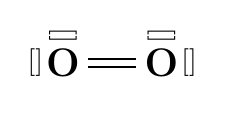
\begin{tikzpicture}[declare function={r=1.0;R=10pt;},baseline={(0pt,-2.5pt)},inner sep=0pt,outer sep=auto]
			\tikzstyle{element_style} = [font=\Large\bfseries, inner sep=3pt]
			% Node trung tâm
			\path(0*r,0) coordinate (A) node[element_style](Oa){O};
			\path(1.25*r,0) coordinate (B) node[element_style](Ob){O};;
			% Vẽ các electron ở các góc ở Oa
			\foreach [count=\i from=1] \g/\c in {90/\mauphu, 180/\mauphu} {
				\path (Oa)--++(\g:R) coordinate (O-\i) 
				node[pos=1,sloped] {\electronH[\c]};
			}
			% Vẽ các electron ở các góc ở Ob
			\foreach [count=\i from=1] \g/\c in {90/\mauphu, 0/\mauphu} {
				\path (Ob)--++(\g:R) coordinate (O-\i) 
				node[pos=1,sloped] {\electronH[\c]};
			}
			%%Vẽ nối đôi
			\draw[double,thick,double distance=2pt](Oa)--(Ob);
		\end{tikzpicture}
	}
\end{bt}
%%%=============BT_12=============%%%
\begin{bt}
	Hãy biểu diễn sự hình thành các cặp electron chung cho phân tử $Cl_2$, $CH_4$.
	Từ đó, viết công thức Lewis của các phân tử này.
	\loigiai{%
	Nguyên tử chlorine (Cl): $[Ne]3s^23p^5$. Mỗi nguyên tử Cl cùng góp 1 electron để tạo một cặp electron chung đạt được cấu hình của khí hiếm.\\
	\begin{tikzpicture}[declare function={r=1;},line cap=round,line join=round,inner sep=0pt]
		\tikzstyle{atom_style} = [font=\Large\bfseries, inner sep=3pt]
		\path (r,0) coordinate (A) node {\congthuce[angle=90,color=\mauphu,type=2][angle=-90,color=\mauphu,type=2][angle=0,color=\maunhan,type=1][angle=180,color=\mauphu,type=2]{Center}{Cl}};
		\path (3*r,0) coordinate (B) node {\congthuce[angle=90,color=\mauphu,type=2][angle=-90,color=\mauphu,type=2][angle=0,color=\mauphu,type=2][angle=180,color=\maunhan,type=1]{Center}{Cl}};
		\path ($(A)!0.5!(B)$) coordinate (C) node[atom_style] {+};
		\path (6*r,0) coordinate (D) node {\congthuce[angle=90,color=\mauphu,type=2][angle=-90,color=\mauphu,type=2][angle=0,color=\maunhan,type=2,radius=12pt][angle=180,color=\mauphu,type=2]{Center}{Cl}};
		\path (6.8*r,0)coordinate (E) node {\congthuce[angle=90,color=\mauphu,type=2][angle=-90,color=\mauphu,type=2][angle=0,color=\mauphu,type=2]{Center}{Cl}};
		\path($(B)!0.5!(D)$) node {$\xrightarrow$};
	\end{tikzpicture}
	\\
	Công thức lewis của $Cl_2$.
	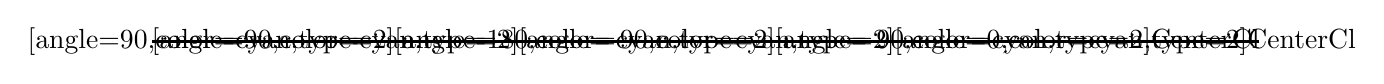
\begin{tikzpicture}[declare function={r=1;},baseline={([yshift=-3pt]current bounding box.base)},outer sep=0pt,inner sep=0pt]
		\path (0,0) node [name = Cla] {\congthuce[angle=90,color=cyan,type=2][angle=180,color=cyan,type=2][angle=-90,color=cyan,type=2]{Center}{Cl}};
		%%%
		\path (1.4,0) node [name = Clb] {\congthuce[angle=90,color=cyan,type=2][angle=-90,color=cyan,type=2][angle=0,color=cyan,type=2]{Center}{Cl}};
		%%%
		\draw[thick] (Cla.east)--(Clb.west);
	\end{tikzpicture}
	\\
	Cấu hình electron:(C): $1s^22s^22p^2$; (H): $1s^1$\\
	4 nguyên tử H và 1 nguyên tử C cùng góp 4 electron để tạo thành 4 cặp electron chung.\\
	\begin{tabular}{|c|c|}
		\hline
		Công thức electron&Công thức Lewis\\
		\hline
			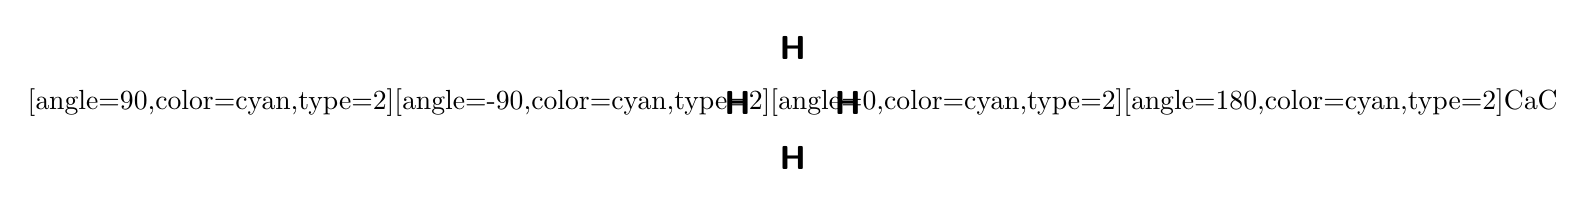
\begin{tikzpicture}[declare function={r=1;},baseline={([yshift=-3pt]current bounding box.base)},outer sep=0pt,inner sep=0pt]
			\tikzstyle{atom_style} = [font=\large\bfseries\sffamily, inner sep=3pt]
			\path (0,0)coordinate (A) node (center) {\congthuce[angle=90,color=cyan,type=2][angle=-90,color=cyan,type=2][angle=0,color=cyan,type=2][angle=180,color=cyan,type=2]{Ca}{C}};
			%%%
			\foreach \g in{90,-90,0,180}{
				\path (center)--++(\g:0.7cm) node[pos=1,atom_style]{H};
			}
		\end{tikzpicture}
		&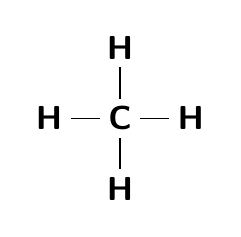
\begin{tikzpicture}[declare function={r=1;},baseline={([yshift=-3pt]current bounding box.base)},outer sep=0pt,inner sep=0pt]
			\tikzstyle{atom_style} = [font=\large\bfseries\sffamily, inner sep=3pt]
			\path (0,0)coordinate (A) node[atom_style] (center) {C};
			%%%
			\foreach[count=\i from=1] \g in{90,-90,0,180}{
				\path (center)--++(\g:0.9cm)  node [pos=1,inner sep=1pt,atom_style](H-\i){H};
				\draw (center)--(H-\i);
			}
		\end{tikzpicture}\\
		\hline
	\end{tabular}
	}
\end{bt}
%%%=============BT_13=============%%%
\begin{bt}
	Hãy biểu diễn sự hình thành các cặp electron chung cho phân tử $C_2H_4$, $C_2H_2$. Từ đó, viết công thức Lewis của các phân tử này.
	\loigiai{
		
	}
\end{bt}
%%%=============BT_14=============%%%
\begin{bt}
	Hãy biểu diễn sự hình thành các cặp electron chung cho phân tử $H_2S$. Từ đó, viết công thức Lewis của phân tử này.
	\loigiai{}
\end{bt}
%%%=============BT_15=============%%%
\begin{bt}
	Dựa theo độ âm điện, hãy cho biết loại liên kết trong các phân tử: $Na_2O$, $H_2O$, $CH_4$, $NaCl$. Cho bảng giá trị độ âm điện
	\begin{center}
		\begin{tabular}{|c|c|c|c|c|c|c|}
			\hline
			Nguyên tố & Na & S & H & C & Cl & O \\
			\hline
			Độ âm điện & $0{,}93$ & $2{,}58$ & $2{,}20$ & $2{,}55$ & $3{,}16$ & $3{,}44$ \\
			\hline
		\end{tabular}
	\end{center}
	\loigiai{}
\end{bt}
%%%=============BT_16=============%%%
\begin{bt}
	Sắp xếp các chất sau theo chiều tăng dần độ phân cực của liên kết: $HCl$, $HF$, $HBr$, $HI$. Biết độ âm điện các nguyên tố được cho ở bảng sau:
	\begin{center}
		\begin{tabular}{|c|c|c|c|c|c|}
			\hline
			Nguyên tố & H & F & Cl & Br & I \\
			\hline
			Độ âm điện & $2{,}20$ & $3{,}98$ & $3{,}16$ & $2{,}96$ & $2{,}66$ \\
			\hline
		\end{tabular}
	\end{center}
	\loigiai{}
\end{bt}
%%%=============BT_17=============%%%
\begin{bt}
	Vẽ sơ đồ biểu diễn liên kết hydrogen giữa hai phân tử $H_2O$.
	\loigiai{}
\end{bt}
%%%=============BT_18=============%%%
\begin{bt}
	Giải thích vì sao nước đá nhẹ và nổi trên mặt nước?
	\loigiai{}
\end{bt}
%%%=============BT_19=============%%%
\begin{bt}
	Cho bảng sau về nhiệt độ sôi và độ tan trong nước của $NH_3$ và $PH_3$
	\begin{center}
		\begin{tabular}{|c|c|c|}
			\hline
			Chất & $NH_3$ & $PH_3$ \\
			\hline
			Nhiệt độ sôi & $-33{,}34^\circ C$ & $-87{,}7^\circ C$ \\
			\hline
			Độ tan & $89{,}9$ g/ $100$ ml ở $0^\circ C$ & $31{,}2$ mg/ $100$ ml ($17^\circ C$) \\
			\hline
		\end{tabular}
	\end{center}
	Giải thích vì sao nhiệt độ sôi và độ tan của $NH_3$ lớn hơn $PH_3$
	\loigiai{}
\end{bt}
%%%=============BT_20=============%%%
\begin{bt}
	Cho bảng nhiệt độ sôi của ethanol và dimethyl ether.
	\begin{center}
		\begin{tabular}{|c|c|c|}
			\hline
			Chất & Khối lượng phân tử & Nhiệt độ sôi \\
			\hline
			ethanol & $46$ & $78{,}3^\circ C$ \\
			\hline
			dimethyl ether & $46$ & $-23^\circ C$ \\
			\hline
		\end{tabular}
	\end{center}
	Hãy giải thích vì sao hai chất có khối lượng phân tử bằng nhau nhưng nhiệt độ sôi lại khác xa nhau.
	\loigiai{}
\end{bt}
%%%=============BT_21=============%%%
\begin{bt}
	Giải thích vì sao nhện nước có thể di chuyển trên mặt nước?
	\loigiai{}
\end{bt}
%%%=============BT_22=============%%%
\begin{bt}
	Cho bảng sau về nhiệt độ nóng chảy, nhiệt độ sôi của các halogen
	\begin{center}
		\begin{tabular}{|c|c|c|c|c|}
			\hline
			Halogen & $F_2$ & $Cl_2$ & $Br_2$ & $I_2$ \\
			\hline
			Trạng thái ở $25^\circ C$ & Khí & Khí & Lỏng & Rắn \\
			\hline
			Nhiệt độ sôi ($^\circ C$) & $-188{,}1$ & $-34{,}1$ & $59{,}2$ & $185{,}5$ \\
			\hline
			Nhiệt độ nóng chảy ($^\circ C$) & $-219{,}6$ & $-101{,}0$ & $-7{,}3$ & $113{,}6$ \\
			\hline
		\end{tabular}
	\end{center}
	Hãy giải thích sự tăng dần nhiệt độ nóng chảy, nhiệt độ sôi của các halogen.
	\loigiai{}
\end{bt}
%%%=============BT_23=============%%%
\begin{bt}
	Giải thích vì sao có thể thu được ethanol ($C_2H_5OH$) bằng phương pháp chưng cất?
	\loigiai{}
\end{bt}
%%%=============BT_24=============%%%
\begin{bt}
	Cho đồ thị biểu diễn nhiệt độ sôi của halides Hãy giải thích xu hướng nhiệt dộ sôi của các halides.
	\loigiai{}
\end{bt}
%%%=============BT_25=============%%%
\begin{bt}
	Giải thích vì sao propanol $\left(CH_3CH_2CH_2OH\right)$ tan trong nước nhutres propan $CH_3CH_2CH_3$ thi không?
	\loigiai{}
\end{bt}
%%%=============BT_26=============%%%
\begin{bt}
	Giải thích vì sao nhiệt độ sôi của butan $\left(36^{\circ} C\right)$ cao hơn so với neopentive $\left(9,5^{\circ} C\right)$?
	\loigiai{}
\end{bt}
%%%=============BT_27=============%%%
\begin{bt}
	Giải thích vì sao $H_2O$ có nhiệt độ sôi $\left(100^{\circ} C\right)$ cao hơn phân tử $NH_3$. $33,34^{\circ} C$?
	\loigiai{}
\end{bt}
%%%=============BT_28=============%%%
\begin{bt}
	Giải thích vì sao thằn lằn có thể bỏ trên trần nhà?
	\loigiai{}
\end{bt}
%%==============Bài tập tự luận Sách BT Cánh diều===========%%%%
%%==============Bai_BT1==============%%%
\begin{bt}
	Hãy giải thích lí do khác nhau về nhiệt độ sôi của các cặp chất có cùng số
	electron sau đây: $CH_3CH_3$ ($184{,}5$ K) và $CH_3-F$ ($194{,}7$ K).
	\loigiai{Phân tử $CH_3-F$ có tương tác giữa các phân tử mạnh hơn do có liên kết C-F phân cực hơn hơn liên kết C-C trong phân tử $CH_3-CH_3$}
\end{bt}
%%==============HetBai_BT1==============%%%

%%==============Bai_BT2==============%%%
\begin{bt}
	Ở điều kiện thường, các khí hiếm tồn tại ở dạng khí đơn nguyên tử.
	Hãy giải thích sự biến đổi nhiệt độ sôi của các khí hiếm từ He tới Rn theo số
	liệu cho trong bảng sau:
	\begin{center}
		\begin{tabular}{|c|c|c|c|c|c|c|}
			\hline
			Khí hiếm & He & Ne & Ar & Kr & Xn & Rn \\
			\hline
			Số hiệu nguyên tử & $2$ & $10$ & $18$ & $36$ & $54$ & $86$ \\
			\hline
			Nhiệt độ sôi ($^\circ$ C) & $-269$ & $-246$ & $-186$ & $-152$ & $-108$ & $-62$ \\
			\hline
		\end{tabular}
	\end{center}
	\loigiai{Do khối lượng nguyên tử tăng dần và theo chiều tăng của Z, số electron và kích thước nguyên tử tăng dần gây nên sự phân cực tạm thời của nguyên tử mạnh hơn nên tương tác van der Waals mạnh dần lên.}
\end{bt}
%%==============HetBai_BT2==============%%%

%%==============Bai_BT3==============%%%
\begin{bt}
	Trong dung dịch, acetic acid có thể tồn tại dạng dimer (hai phân tử kết hợp) do sự hình thành liên kết hydrogen giữa hai phân tử. Hãy vẽ sơ đồ biểu diễn liên kết hydrogen giữa hai phân tử acetic acid hình thành dimer.
	\loigiai{}
\end{bt}
%%==============HetBai_BT3==============%%%

%%==============Bai_BT4==============%%%
\begin{bt}
	Hãy giải thích sự biến đổi về nhiệt độ nóng chảy của dãy hydrogen halide sau.
	\begin{center}
		\begin{tabular}{|c|c|c|c|c|}
			\hline
			Halogen halide & HF & HCl & HBr & HI \\
			\hline
			Nhiệt độ nóng chảy ($^\circ$ C) & $-83{,}1$ & $-114{,}8$ & $-88{,}5$ & $-50{,}8$ \\
			\hline
		\end{tabular}
	\end{center}
	\loigiai{Giữa các phân tử HF có liên kết hydrogen nên nhiệt độ nóng chảy cao hơn so với HCl. Từ HCl tới HI do kích thước nguyên tử halogen tăng, tương tác van der Waals giữa các phân tử tăng nên nhiệt độ nóng chảy tăng.}
\end{bt}
%%==============HetBai_BT4==============%%%

%%==============Bai_BT5==============%%%
\begin{bt}
	Nhiệt độ sôi của ba hợp chất được cho trong bảng sau:
	\begin{center}
		\begin{tabular}{|c|c|c|}
			\hline
			Hợp chất & Khối lượng phân tử (g mol$^{-1}$) & Nhiệt độ sôi ($^\circ$C) \\
			\hline
			2-hexanone & $100{,}16$ & $128{,}0$ \\
			\hline
			heptane & $100{,}20$ & $98{,}0$ \\
			\hline
			1-hexanol & $102{,}17$ & $156{,}0$ \\
			\hline
		\end{tabular}
	\end{center}
	Không cần tra cứu cấu trúc, em hãy trả lời các câu hỏi sau về ba hợp chất này:
	\begin{enumerate}
		\item Hợp chất nào có thể hình thành liên kết hydrogen?
		\item Hợp chất nào phân cực nhưng không hình thành liên kết hydrogen?
		\item Hợp chất nào ít phân cực, không tạo liên kết hydrogen?
	\end{enumerate}
	\loigiai{Ba chất có khối lượng phân tử tương đương nhau nên chất có nhiệt độ sôi cao nhất là chất có thể hình thành liên kết hydrogen, đó là 1-hexanol.
		
		Chất có phân tử phân cực sẽ có liên kết van der Waals giữa các phân tử mạnh hơn, có nhiệt độ sôi xếp thứ hai (ảnh hưởng của liên kết hydrogen tới nhiệt độ sôi là mạnh hơn tương tác van der Waals), do đó chất phân cực là 2-hexanone.
		Còn lại là heptane.}
\end{bt}
%%==============HetBai_BT5==============%%%


%%=======Bài tập tự luận sách chân trời sáng tao==============%%%%
%%==============Bai_BT1==============%%%
\begin{bt}
	Biểu diễn liên kết hydrogen giữa các phân tử sau:
	\begin{enumerate}
		\item methanol ($CH_3OH$) và nước.
		\item ethylene glycol ($HOCH_2CH_2OH$) và nước.
	\end{enumerate}
	Từ đó nhận xét tính tan của methanol và ethylene glycol trong nước.
	\loigiai{}
\end{bt}
%%==============HetBai_BT1==============%%%

%%==============Bai_BT2==============%%%
\begin{bt}
	Ethylene glycol ($HOCH_2CH_2OH$) là một chất chống đông trong công nghiệp ô tô, hàng không do có khả năng can thiệp vào liên kết hydrogen của nước, làm các phân tử nước khó liên kết hơn, khiến nước khó đóng băng hơn.
	Biểu diễn liên kết hydrogen liên phân tử và nội phân tử trong ethylene glycol.
	\loigiai{}
\end{bt}
%%==============HetBai_BT2==============%%%

%%==============Bai_BT3==============%%%
\begin{bt}
	Hãy so sánh tương tác van der Waals với liên kết ion.
	\loigiai{Tương tác van der Waals và liên kết ion đều là các lực hút tĩnh điện. Tuy nhiên, tương tác van der Waals là lực hút tĩnh điện giữa các phân tử trung hoà nên yếu hơn nhiều so với liên kêt ion là lực hút tĩnh điện giữa các ion trái dấu.}
\end{bt}
%%==============HetBai_BT3==============%%%

%%==============Bai_BT4==============%%%
\begin{bt}
	Thiết bị chụp cộng hưởng từ hạt nhân (NMR) sử dụng nitrogen lỏng để làm mát nam châm siêu dẫn. Nitrogen lỏng sôi ở $–195{,}8$ °C. Dự đoán nhiệt độ sôi của oxygen lỏng sẽ cao hay thấp hơn so với nitrogen lỏng? Giải thích.
	\loigiai{Oxygen có khối lượng phân tử cao hơn nitrogen, do đó tương tác van der Waals giữa các phân tử oxygen mạnh hơn so với nitrogen. Kết quả oxygen lỏng có nhiệt độ sôi cao hơn nitrogen lỏng. Thật vậy, oxygen lỏng sôi ở $-183^{\circ} \mathrm{C}$, trong khi nitrogen lỏng sôi ở $-195,8^{\circ} \mathrm{C}$.}
\end{bt}
%%==============HetBai_BT4==============%%%

%%==============Bai_BT5==============%%%
\begin{bt}
	Giải thích vì sao các tương tác van der Waals giữa các phân tử có kích thước lớn lại mạnh hơn so với các phân tử có kích thước nhỏ.
	\loigiai{Phân tử có kích thước lớn thường đi đôi với nhiều electron. Chính vì vậy khả năng tạo các lưỡng cực tức thời và lưỡng cực cảm ứng của các phân tử có kích thước lớn cũng nhiều hơn, từ đó tương tác van der Waals giữa các phân tử lớn cũng mạnh hơn, nên các phân tử có kích thước lớn "dính" với nhau hơn so với các phân tử có kích thước nhỏ.}
\end{bt}
%%==============HetBai_BT5==============%%%

%%==============Bai_BT6==============%%%
\begin{bt}
	Giải thích tại sao ở điều kiện thường, các nguyên tố trong nhóm halogen như fluorine và chlorine ở trạng thái khí, còn bromine ở trạng thái lỏng và iodine ở trạng thái rắn.
	\loigiai{Khi đi từ $\mathrm{F}_2$ đến $\mathrm{I}_2$, do khối lượng phân tử các halogen tăng dần làm tương tác van der Waals giữa các phân tử halogen cũng tăng dần, kết quả các phân tử halogen "dính" với nhau chặt hơn, nên fluorine và chlorine ở trạng thái khi, còn bromine ở trạng thái lỏng và iodine ở trạng thái rắn.}
\end{bt}
%%==============HetBai_BT6==============%%%

%%==============Bai_BT7==============%%%
\begin{bt}
	Nhiệt độ sôi của các hợp chất với hydrogen của các nguyên tố nhóm VA, VIA và VIIA được biểu diễn qua đồ thị sau:
	\begin{enumerate}
		\item Giải thích nhiệt độ sôi cao bất thường của các hợp chất với hydrogen của các nguyên tố đầu tiên trong mỗi nhóm.
		\item Nhận xét nhiệt độ sôi của các hợp chất với hydrogen của các nguyên tố còn lại ở mỗi nhóm và giải thích nguyên nhân sự biến đổi nhiệt độ sôi của chúng.
	\end{enumerate}
	\loigiai{%
	\begin{enumerate}[a)]
		\item  Các nguyên tố đầu tiên trong mỗi nhóm VA, VIA, VIIA $(\mathrm{N}, \mathrm{O}, \mathrm{F})$ có kích thước nhỏ và có độ âm điện lớn, kết quả trong các hợp chất $\mathrm{NH}_3 ; \mathrm{H}_2 \mathrm{O} ; \mathrm{HF}$ xuất hiện liên kết hydrogen liên phân tử làm các hợp chất này có nhiệt độ sôi cao bất thường so với các hợp chất còn lại trong mỗi nhóm.
		\item  Hợp chất với hydrogen của các nguyên tố còn lại trong mỗi nhóm có nhiệt độ sôi tăng dần khi khối lượng phân tử của chúng tăng. Vì khi khối lượng phân tử tăng, tương tác van der Waals giữa các phân tử trong hợp chất cũng tăng làm các phân tử "dính" với nhau chặt hơn, dẫn đến nhiệt độ sôi của chúng dần cao hơn.
	\end{enumerate}
	}
\end{bt}
%%==============HetBai_BT7==============%%%

%%==============Bai_BT8==============%%%
\begin{bt}
	So sánh nhiệt độ nóng chảy và nhiệt độ sôi của pentane ($CH_3CH_2CH_2CH_2CH_3$) và neopentane ($(CH_3)_4C$). Giải thích nguyên nhân sự khác biệt trên.
	\loigiai{Hai hợp chất đã cho có cùng công thức phân tử, tức cùng khối lượng phân tử. Tuy nhiên phân tử neopentane có dạng hình cầu nên diện tích bề mặt tiếp xúc giữa các phân tử neopentane nhỏ hơn so với các phân tử pentane. Kết quả các phân tử pentane \lq\lq dính\rq\rq\ với nhau hơn so với các phân tử neopentane nên nhiệt độ nóng chảy và nhiệt độ sôi của pentane $\left(-130^{\circ} \mathrm{C}\right.$ và $\left.36,0^{\circ} \mathrm{C}\right)$, cao hơn so với neopentane $\left(-16,6^{\circ} \mathrm{C}\right.$ và $\left.9,5^{\circ} \mathrm{C}\right)$.}
\end{bt}
%%==============HetBai_BT8==============%%%

%%==============Bai_BT9==============%%%
\begin{bt}
	Giải thích vì sao tetrachloromethane ($CCl_4$) tuy là phân tử không cực nhưng có nhiệt độ sôi cao hơn trichloromethane ($CHCl_3$) là phân tử có cực.
	\loigiai{$\mathrm{CHCl}_3$ là một phân tử phân cực, trong khi $\mathrm{CCl}_4$ là một phân tử không phân cực. Như vậy, $\mathrm{CHCl}_3$ đáng lý phải có nhiệt độ sôi cao hơn $\mathrm{CCl}_4$. Tuy nhiên thực tế $\mathrm{CCl}_4$ lại có nhiệt độ sôi cao là $76,8^{\circ} \mathrm{C}$, cao hơn so với $\mathrm{CHCl}_3$ là $61,2^{\circ} \mathrm{C}$. Điều này là do phân tử $\mathrm{CCl}_4$ có kích thước lớn hơn $\mathrm{CHCl}_3$ nên có số electron cũng nhiều hơn $\mathrm{CHCl}_3$, do đó tương tác van der Waals giữa các phân tử $\mathrm{CCl}_4$ mạnh hơn so với $\mathrm{CHCl}_3$ làm cho $\mathrm{CCl}_4$ có nhiệt độ sôi cao hơn $\mathrm{CHCl}_3$.}
\end{bt}
%%==============HetBai_BT9==============%%%


%%Bài tập tụ luận sách bài tập KNTTVCS=================%%%
%%==============Bai_BT1==============%%%
\begin{bt}
	Cho các chất sau: $C_2H_6$; $CH_3OH$; $CH_3COOH$.
	Chất nào có thể tạo được liên kết hydrogen? Vì sao?
	\loigiai{$\mathrm{CH}_3 \mathrm{OH}$ và $\mathrm{CH}_3 \mathrm{COOH}$ chứa nguyên tử O có độ âm điện lớn $(3,44)$ và nguyên tử H liên kết với nguyên tử O trong nhóm -OH là nguyên tử hydrogen linh động tạo ra liên kết hydrogen:
		\[\cdots \mathrm{O}-\mathrm{H} \cdots \mathrm{O}-\mathrm{H} \cdots\]}
\end{bt}
%%==============HetBai_BT1==============%%%

%%==============Bai_BT2==============%%%
\begin{bt}
	Khối lượng mol (g/mol) của nước, ammonia và methane lần lượt bằng 18,17 và 16. Nước sôi ở $100^\circ C$, còn ammonia sôi ở $-33{,}35^\circ C$ và methane sôi ở $-161{,}58^\circ C$. Giải thích vì sao các chất trên có khối lượng mol xấp xỉ nhau nhưng nhiệt độ sôi của chúng lại chênh lệch nhau.
	\loigiai{Nhiệt độ sôi của $H_2O$ lớn hơn rất nhiều so với $NH_3$ và $CH_4$ vì phân tử $H_2O$ và $NH_3$ có liên kết hydrogen liên phân tử (còn $CH_4$ không có); do độ âm điện O > N nên liên kết hydrogen trong $H_2O$ bền hơn trong $NH_3$.
	}
\end{bt}
%%==============HetBai_BT2==============%%%

%%==============Bai_BT3==============%%%
\begin{bt}
	Trong dung dịch ethanol ($C_2H_5OH$) có những kiểu liên kết hydrogen nào? Kiểu nào bền nhất và kém bền nhất? Mô tả bằng hình vẽ.
	\loigiai{Dung dịch ethanol có $C_2H_5OH$ và $H_2O$, cả hai phân tử này đều chứa nguyên tử O có độ âm điện lớn ($3{,}44$) và nguyên tử H liên kết với nguyên tử O trong nhóm $-OH$ là nguyên tử hydrogen linh động tạo ra liên kết hydrogen.
	Có bốn kiểu liên kết hydrogen trong dung dịch ethanol: alcohol - alcohol; nước – nước; alcohol – nước và nước – alcohol.
		
	Liên kết hydrogen càng bền khi nguyên tử có độ âm điện lớn hơn và nguyên tử H linh động hơn. Trong bốn kiểu trên: kiểu bền nhất là liên kết giữa H của nước với O của alcohol (nước – alcohol). Kiểu kém bền nhất là liên kết giữa H của alcohol với O của alcohol (alcohol - alcohol).}
\end{bt}
%%==============HetBai_BT3==============%%%

%%==============Bai_BT4==============%%%
\begin{bt}
	Trong phân tử nước và ammonia, phân tử nào có thể tạo nhiều liên kết hydrogen hơn? Vì sao?
	\loigiai{\begin{itemize}
			\item  Số liên kết hydrogen trung bình được tạo thành trên mỗi phân tử phụ thuộc vào:
			\begin{itemize}
				\item  Số nguyên tử hydrogen liên kết với F, O hoặc N trong phân tử.
				\item  Số lượng các cặp electron chưa liên kết có mặt trên F, O, N.
			\end{itemize}
			\item  Mỗi phân tử nước có hai nguyên tử hydrogen và hai cặp electron chưa liên kết nên phân tử nước có nhiều liên kết hydrogen với các phân tử nước khác. Nó có mức trung bình là hai liên kết hydrogen trên mỗi phân tử.
			\item  Ammonia có ít liên kết hydrogen hơn nước. Trung bình nó có thể hình thành chỉ một liên kết hydrogen trên mỗi phân tử. Mặc dù mỗi phân tử ammonia có ba nguyên tử hydrogen gắn với nguyên tử nitrogen, nhưng nó chỉ có một cặp electron duy nhất có thể tham gia vào quá trình hình thành liên kết hydrogen.
	\end{itemize}}
\end{bt}
%%==============HetBai_BT4==============%%%

%%==============Bai_BT5==============%%%
\begin{bt}
	Dầu mỏ chứa hỗn hợp nhiều hydrocarbon như: octane ($C_8H_{18}$) có trong xăng; butane ($C_4H_{10}$) có trong gas. Khi chưng cất dầu mỏ, octane hay butane sẽ bay hơi trước? Giải thích.
	\loigiai{Khi chưng cất dầu mỏ, butane sẽ bay hơi trước octane. Vì octane ($M = 114$) có phân tử khối lớn hơn butane ($M = 58$) nên có nhiệt độ sôi cao hơn.}
\end{bt}
%%==============HetBai_BT5==============%%%

%%==============Bai_BT6==============%%%
\begin{bt}
	Cho các chất và các trị số nhiệt độ sôi ($^\circ C$) sau: $H_2O$, $H_2S$, $H_2Se$, $H_2Te$ và $-42$; $-2$; $100$; $-61$.
	Ghép các trị số nhiệt độ sôi vào mỗi chất sao cho phù hợp và giải thích.
	\loigiai{\begin{itemize}
			\item  Giá trị nhiệt độ sôi của từng chất:
			$H_2O$ (100 °C); $H_2S$ (-61 °C); $H_2Se$ (-42 °C) và $H_2Te$ (-2 °C).
			\item  \indam[\maunhan]{Giải thích:} sự tăng nhiệt độ sôi từ $H_2S$ đến $H_2Te$ là do khối lượng phân tử tăng lên. Nếu $H_2O$ chỉ có lực van der Waals giữa các phân tử thì nhiệt độ sôi của nó dự đoán vào khoảng $-80^\circ C$. Tuy nhiên, nhiệt độ sôi của $H_2O$ là $100^\circ C$, cao hơn nhiều, đó là vì phân tử $H_2O$ còn có liên kết hydrogen liên phân tử, làm cho liên kết giữa các phân tử $H_2O$ bền vững hơn.
	\end{itemize}}
\end{bt}
%%==============HetBai_BT6==============%%%
\Closesolutionfile{ansbt}
\Closesolutionfile{ansbth}
%\bangdapanSA{AnsBT-C03B04_LKH_TTVANDERWALLS}

%%=======================PHẦN TRẮC NGHIỆM======================%%%%
\phan{Trắc nghiệm nhiều lựa chọn}
%=============SOẠN EX===============%%%
\Opensolutionfile{ansex}[Ans/LGEX-C03B04_LKH_TTVANDERWALLS]
\Opensolutionfile{ans}[Ans/Ans-C03B04_LKH_TTVANDERWALLS]

%Câu hỏi trắc nghiệm sách bài tập Cánh diều
%==============Cau_1==============%%%
\begin{ex}
	Phát biểu nào sau đây là \textbf{đúng}?
	\choice
	{Bất kì phân tử nào có chứa nguyên tử hydrogen cũng có thể tạo liên kết hydrogen với phân tử cùng loại}
	{Liên kết hydrogen là liên kết hình thành do sự góp chung cặp electron hoá trị giữa nguyên tử hydrogen và nguyên tử có độ âm điện lớn}
	{Liên kết hydrogen là loại liên kết yếu nhất giữa các phân tử}
	{\True Ảnh hưởng của liên kết hydrogen tới nhiệt độ sôi và nhiệt độ nóng chảy của chất là mạnh hơn ảnh hưởng của tương tác van der Waals}
	\loigiai{}
\end{ex}
%==============HetCau_1==============%%%

%==============Cau_2==============%%%
\begin{ex}
	Cho các phân tử: $H_2O$, $NH_3$, $HF$, $H_2S$, $CO_2$, $HCl$. Số phân tử có thể tạo liên kết hydrogen với phân tử cùng loại là
	\choice
	{\True $3$}
	{$4$}
	{$5$}
	{$6$}
	\loigiai{Chỉ có $\mathrm{H}_2 \mathrm{O}, \mathrm{NH}_3, \mathrm{HF}$ mới tạo được liên kết hydro với các phân tử cùng loại; còn $\mathrm{H}_2 \mathrm{S}, \mathrm{CO}_2, \mathrm{HCl}$ thì không.}
\end{ex}
%==============HetCau_2==============%%%

%==============Cau_3==============%%%
\begin{ex}
	Thứ tự nào sau đây thể hiện độ mạnh giảm dần của các loại liên kết?
	\choice
	{\True Liên kết ion > liên kết cộng hoá trị > liên kết hydrogen > tương tác van der Waals}
	{Liên kết ion > liên kết cộng hoá trị > tương tác van der Waals > liên kết hydrogen}
	{Liên kết cộng hoá trị > liên kết ion > liên kết hydrogen > tương tác van der Waals}
	{Tương tác van der Waals > liên kết hydrogen > liên kết cộng hoá trị > liên kết ion}
	\loigiai{}
\end{ex}
%==============HetCau_3==============%%%

%==============Cau_4==============%%%
\begin{ex}
	Giữa các nguyên tử He có thể có loại liên kết nào?
	\choice
	{Liên kết cộng hoá trị}
	{Liên kết hydrogen}
	{\True Tương tác van der Waals}
	{Không có bất kì liên kết nào}
	\loigiai{Giữa các phân tử không phân cực hoặc giữa các nguyên tử khí hiếm vẫn có thời điểm xuất hiện sự phân cực tạm thời (do nguyên tử chứa các hạt mang điện là proton và electron), do đó luôn có tương tác van der Waals.
	}
\end{ex}
%==============HetCau_4==============%%%

%==============Cau_5==============%%%
\begin{ex}
	Quy tắc octet không được sử dụng khi xem xét sự hình thành của hai loại liên kết hoặc tương tác nào sau đây?
	\begin{enumerate}[(1)]
		\item  Liên kết cộng hoá trị.
		\item  Liên kết ion.
		\item  Liên kết hydrogen.
		\item  Tương tác van der Waals.
	\end{enumerate}
	\choice
	{(1) và (2)}
	{(2) và (3)}
	{(1) và (3)}
	{\True (3) và (4)}
	\loigiai{}
\end{ex}
%==============HetCau_5==============%%%

%==============Cau_6==============%%%
\begin{ex}
	Nếu giữa phân tử chất tan và dung môi có thể tạo thành liên kết hydrogen
	hoặc có tương tác van der Waals càng mạnh với nhau thì càng tan tốt vào nhau.
	Lí do nào sau đây là phù hợp để giải thích dầu hỏa (thành phần chính là
	hydrocarbon) không tan trong nước?
	\choice
	{Cả nước và dầu đều là các phân tử có cực}
	{\True Nước là phân tử phân cực và dầu là không/ít phân cực}
	{Nước là phân tử không phân cực và dầu là phân cực}
	{Cả nước và dầu đều không phân cực}
	\loigiai{}
\end{ex}
%==============HetCau_6==============%%%

%==============Cau_7==============%%%
\begin{ex}
	Ethanol tan vô hạn trong nước do
	\choice
	{cả nước và ethanol đều là phân tử phân cực}
	{\True nước và ethanol có thể tạo liên kết hydrogen với nhau}
	{ethanol có thể tạo liên kết hydrogen với các phân tử ethanol khác}
	{ethanol và nước có tương tác van der Waals mạnh}
	\loigiai{}
\end{ex}
%==============HetCau_7==============%%%

%==============Cau_8==============%%%
\begin{ex}
	Chất nào trong số các chất sau tồn tại ở thể lỏng trong điều kiện thường?
	\choice
	{\True $CH_3OH$}
	{$CF_4$}
	{$SiH_4$}
	{$CO_2$}
	\loigiai{Giữa các phân tử $\mathrm{CH}_3 \mathrm{OH}$ có thể hinh thành liên kết hydrogen.}
\end{ex}
%==============HetCau_8==============%%%

%==============Cau_9==============%%%
\begin{ex}
	Dựa vào liên kết giữa các phân tử, hãy cho biết halogen nào sau đây có nhiệt
	độ sôi cao nhất.
	\choice
	{$F_2$}
	{$Cl_2$}
	{$Br_2$}
	{\True $I_2$}
	\loigiai{Do $I_2$ có khối lượng phân tử lớn nhất và đồng thời có kích thước lớn nhất nên tương tác van der Waals giữa các phân tử mạnh hơn. 
	}
\end{ex}
%==============HetCau_9==============%%%


%Câu hỏi trắc nghiệm sách bài tập chân trời sáng tạo 
%==============Cau_1==============%%%
\begin{ex}
	Hợp chất nào sau đây tạo được liên kết hydrogen liên phân tử?
	\choice
	{$H_2S$}
	{$PH_3$}
	{$HI$}
	{\True $CH_3OH$}
	\loigiai{}
\end{ex}
%==============HetCau_1==============%%%

%==============Cau_2==============%%%
\begin{ex}
	Mặc dù chlorine có độ âm điện là $3{,}16$ xấp xỉ với nitrogen là $3{,}04$ nhưng giữa
	các phân tử HCl không tạo được liên kết hydrogen với nhau, trong khi giữa
	các phân tử $NH_3$ tạo được liên kết hydrogen với nhau, nguyên nhân là do
	\choice
	{độ âm điện của chlorine nhỏ hơn của nitrogen}
	{phân tử $NH_3$ chứa nhiều nguyên tử hydrogen hơn phân tử HCl}
	{tổng số nguyên tử trong phân tử $NH_3$ nhiều hơn so với phân tử HCl}
	{\True kích thước nguyên tử chlorine lớn hơn nguyên tử nitrogen nên mật độ điện
		tích âm trên chlorine không đủ lớn để hình thành liên kết hydrogen}
	\loigiai{}
\end{ex}
%==============HetCau_2==============%%%

%==============Cau_3==============%%%
\begin{ex}
	Sơ đồ nào sau đây thể hiện đúng liên kết hydrogen giữa 2 phân tử hydrogen
	fluoride (HF)?
	\choice
	{\True $H^{\delta+}-F^{\delta-}\ldots H^{\delta+}-F^{\delta-}$}
	{$H^{\delta+}-F^{\delta+}\ldots H^{\delta-}-F^{\delta-}$}
	{$H^{\delta-}-F^{\delta+}\ldots H^{\delta-}-F^{\delta+}$}
	{$H^{\delta+}-F^{\delta-}\ldots H^{\delta+}-F^{\delta+}$}
	\loigiai{}
\end{ex}
%==============HetCau_3==============%%%

%==============Cau_4==============%%%
\begin{ex}
	Điều nào sau đây đúng khi nói về liên kết hydrogen liên phân tử?
	\choice
	{\True Là lực hút tĩnh điện giữa nguyên tử H (thường trong các liên kết H-F, H-N, H-O ở phân tử này) với một trong các nguyên tử có độ âm điện mạnh
		(thường là N, O, F) ở một phân tử khác}
	{Là lực hút giữa các phân tử khác nhau}
	{Là lực hút tĩnh điện giữa các ion trái dấu}
	{Là lực hút giữa các nguyên tử trong một hợp chất cộng hoá trị}
	\loigiai{Liên kết hydrogen liên phân tử là lực hút tĩnh điện giữa nguyên tử H (thường trong các liên kết $\mathrm{H}-\mathrm{F} ; \mathrm{H}-\mathrm{N} ; \mathrm{H}-\mathrm{O}$ ở phân tử này) với một trong các nguyên tử có độ âm điện mạnh (thường là $\mathrm{N} ; \mathrm{O} ; \mathrm{F}$ ) ở một phân tử khác.}
\end{ex}
%==============HetCau_4==============%%%

%==============Cau_5==============%%%
\begin{ex}
	Điều nào sau đây đúng khi nói về liên kết hydrogen nội phân tử?
	\choice
	{Là lực hút giữa các proton của nguyên tử này với các electron ở nguyên tử khác}
	{\True Là lực hút tĩnh điện giữa nguyên tử H (thường trong các liên kết H-F, H-N, H-O) ở một phân tử với một trong các nguyên tử có độ âm điện mạnh (thường là N, O, F) ở ngay chính phân tử đó}
	{Là lực hút giữa các ion trái dấu}
	{Là lực hút giữa các phân tử có chứa nguyên tử hydrogen}
	\loigiai{Liên kết hydrogen nội phân tử là lực hút tĩnh điện giửa nguyên tử $H$ ( thưởng trong các liên kết $\mathrm{H}-\mathrm{F} ; \mathrm{H}-\mathrm{N} ; \mathrm{H}-\mathrm{O}$ ) ở một phân tử với một trong các nguyên tử có độ âm điện manh (thường là $\mathrm{N} ; \mathrm{O} ; \mathrm{F}$ ) ở ngay chính phân tử đó.}
\end{ex}
%==============HetCau_5==============%%%

%==============Cau_6==============%%%
\begin{ex}
	Tương tác van der Waals xuất hiện là do sự hình thành các lưỡng cực tạm thời cũng như các lưỡng cực cảm ứng. Các lưỡng cực tạm thời xuất hiện là do sự chuyển động của
	\choice
	{các nguyên tử trong phân tử}
	{\True các electron trong phân tử}
	{các proton trong hạt nhân}
	{các neutron và proton trong hạt nhân}
	\loigiai{Tương tác van der Waals xuất hiện là do sự hình thành các lưỡng cực tạm thời cũng như các lưỡng cực cảm ứng. Các lưỡng cực tạm thởi xuất hiện là đo sự chuyển động của các electron trong phân tử, đỏ là lúc electron tập trung về một phía trong phân tử.}
\end{ex}
%==============HetCau_6==============%%%

%==============Cau_7==============%%%
\begin{ex}
	Trong các khí hiếm sau, khí hiếm có nhiệt độ sôi cao nhất là
	\choice
	{Ne}
	{\True Xe}
	{Ar}
	{Kr}
	\loigiai{Do có khối lượng phân tử lớn nhất nên tương tác van der Waals giữa các phân tử Xe là lớn nhất, dẫn đến khi hiếm Xe có nhiệt độ sồi cao nhất.}
\end{ex}
%==============HetCau_7==============%%%

%Cau hỏi trắc nghiệm sách bài tập kết nối tri thức
%==============Cau_1==============%%%
\begin{ex}
	Liên kết hydrogen là loại liên kết hoá học được hình thành giữa các
	nguyên tử nào sau đây?
	\choice
	{Phi kim và hydrogen trong hai phân tử khác nhau}
	{Phi kim và hydrogen trong cùng một phân tử}
	{Phi kim có độ âm điện lớn và nguyên tử hydrogen}
	{\True $F$, $O$, $N$, $\ldots$ có độ âm điện lớn, đồng thời có cặp electron hoá trị chưa liên kết
		và nguyên tử hydrogen linh động}
	\loigiai{}
\end{ex}
%==============HetCau_1==============%%%

%==============Cau_2==============%%%
\begin{ex}
	Tương tác van der Waals được hình thành do
	\choice
	{tương tác tĩnh điện lưỡng cực – lưỡng cực giữa các nguyên tử}
	{tương tác tĩnh điện lưỡng cực – lưỡng cực giữa các phân tử}
	{\True tương tác tĩnh điện lưỡng cực – lưỡng cực giữa các nguyên tử hay phân tử}
	{lực hút tĩnh điện giữa các phân tử phân cực}
	\loigiai{}
\end{ex}
%==============HetCau_2==============%%%

%==============Cau_3==============%%%
\begin{ex}
	Chất nào sau đây có thể tạo liên kết hydrogen?
	\choice
	{$PF_3$}
	{$CH_4$}
	{\True $CH_3OH$}
	{$H_2S$}
	\loigiai{}
\end{ex}
%==============HetCau_3==============%%%

%==============Cau_4==============%%%
\begin{ex}
	Chất nào sau đây *không* thể tạo được liên kết hydrogen?
	\choice
	{$H_2O$}
	{\True $CH_4$}
	{$CH_3OH$}
	{$NH_3$}
	\loigiai{}
\end{ex}
%==============HetCau_4==============%%%

%==============Cau_5==============%%%
\begin{ex}
	Tương tác van der Waals tồn tại giữa những
	\choice
	{ion}
	{hạt proton}
	{hạt neutron}
	{\True phân tử}
	\loigiai{}
\end{ex}
%==============HetCau_5==============%%%

%==============Cau_6==============%%%
\begin{ex}
	Cho các chất sau: $F_2$, $Cl_2$, $Br_2$, $I_2$.
	Chất có nhiệt độ nóng chảy thấp nhất là
	\choice
	{\True $F_2$}
	{$Cl_2$}
	{$Br_2$}
	{$I_2$}
	\loigiai{}
\end{ex}
%==============HetCau_6==============%%%

%==============Cau_7==============%%%
\begin{ex}
	Cho các chất sau: $F_2$, $Cl_2$, $Br_2$, $I_2$.
	Chất có nhiệt độ sôi cao nhất là
	\choice
	{$F_2$}
	{$Cl_2$}
	{$Br_2$}
	{\True $I_2$}
	\loigiai{}
\end{ex}
%==============HetCau_7==============%%%

%==============Cau_8==============%%%
\begin{ex}
	Dãy chất nào sau đây xếp theo thứ tự nhiệt độ sôi tăng dần?
	\choice
	{$H_2O$, $H_2S$, $CH_4$}
	{$H_2S$, $CH_4$, $H_2O$}
	{$CH_4$, $H_2O$, $H_2S$}
	{\True $CH_4$, $H_2S$, $H_2O$}
	\loigiai{}
\end{ex}
%==============HetCau_8==============%%%

%==============Cau_9==============%%%
\begin{ex}
	Cho các khí hiếm sau: He, Ne, Ar, Kr, Xe.
	Khí hiếm có nhiệt độ nóng chảy thấp nhất và cao nhất lần lượt là
	\choice
	{Xe và He}
	{Ar và Ne}
	{\True He và Xe}
	{He và Kr}
	\loigiai{}
\end{ex}
%==============HetCau_9==============%%%

%==============Cau_10==============%%%
\begin{ex}
	Cho các chất sau: $C_2H_6$; $H_2O$; $NH_3$; $PF_3$; $C_2H_5OH$.
	Số chất tạo được liên kết hydrogen là
	\choice
	{$2$}
	{\True $3$}
	{$4$}
	{$5$}
	\loigiai{}
\end{ex}
%==============HetCau_10==============%%%

%==============Cau_11==============%%%
\begin{ex}
	Giữa $H_2O$ và $HF$ có thể tạo ra ít nhất bao nhiêu kiểu liên kết hydrogen?
	\choice
	{$2$}
	{$3$}
	{\True $4$}
	{$5$}
	\loigiai{}
\end{ex}
%==============HetCau_11==============%%%

%==============Cau_12==============%%%
\begin{ex}
	Nhiệt độ sôi của từng chất methane, ethane, propane và butane là một trong bốn nhiệt độ sau: $0^\circ C$; $-164^\circ C$; $-42^\circ C$ và $-88^\circ C$.
	Nhiệt độ sôi $-88^\circ C$ là của chất nào sau đây?
	\choice
	{methane}
	{propane}
	{\True ethane}
	{butane}
	\loigiai{}
\end{ex}
%==============HetCau_12==============%%%
\Closesolutionfile{ans}
\Closesolutionfile{ansex}
%\bangdapan{Ans-C03B04_LKH_TTVANDERWALLS}
\phan{Trắc nghiệm đúng /sai}
%%%=============SOẠN EXTF===============%%%
\Opensolutionfile{ansex}[Ans/LGTF-C03B04_LKH_TTVDW]
\Opensolutionfile{ansbook}[Ansbook/AnsTF-C03B04_LKH_TTVDW]
\Opensolutionfile{ans}[Ans/Tempt-C03B04_LKH_TTVDW]
%%%%=================EX_01====================%%%%
\begin{ex}
	Trong các chất sau, chất có khả năng tạo liên kết hydrogen giữa các phân tử là:
	\choiceTF[t]
	{\True $ H_2O, NH_3, HF $}
	{$ CH_4, CCl_4, SiH_4 $}
	{\True $ HF, H_2O, H_2S $}
	{$ HCl, HBr, HI $}
	\loigiai{
		\begin{itemchoice}[T1,F2,T3,F4]
			\itemch $ H_2O, NH_3, HF $ đều có nguyên tử H liên kết với các nguyên tử có độ âm điện lớn (O, N, F), cho phép tạo liên kết hydrogen mạnh.
			\itemch Các chất như $ CH_4, CCl_4, SiH_4 $ không có liên kết H với nguyên tố có độ âm điện lớn, nên không hình thành liên kết hydrogen.
			\itemch $ HF, H_2O $ có khả năng tạo liên kết hydrogen mạnh; $ H_2S $ tạo liên kết yếu hơn do độ âm điện của S thấp.
			\itemch $HCl, HBr, HI $ không tạo liên kết hydrogen đáng kể vì độ âm điện của Cl, Br, I thấp hơn nhiều so với O, N, F.
		\end{itemchoice}
	}
\end{ex}

%%%%=================EX_02====================%%%%
\begin{ex}
	Liên kết hydrogen đóng vai trò quan trọng trong tính chất của các hợp chất.
	\choiceTF[t]
	{\True Nhiệt độ sôi của nước cao do liên kết hydrogen}
	{\True ADN duy trì cấu trúc nhờ liên kết hydrogen giữa các base}
	{$H_2S$ có nhiệt độ sôi cao hơn $H_2O$ nhờ liên kết hydrogen}
	{\True Rượu ethanol có khả năng tạo liên kết hydrogen với nước}
	\loigiai{
		\begin{itemchoice}[T1,T2,F3,T4]
			\itemch Liên kết hydrogen bền vững làm tăng nhiệt độ sôi của nước.
			\itemch Trong ADN, liên kết hydrogen tạo sự gắn kết giữa các base nitơ.
			\itemch $H_2S$ không tạo liên kết hydrogen mạnh như $H_2O$, nhiệt độ sôi thấp hơn.
			\itemch Rượu ethanol tạo liên kết hydrogen giữa nhóm OH và nước.
		\end{itemchoice}
	}
\end{ex}

%%%%=================EX_03====================%%%%
\begin{ex}
	Tương tác van der Waals có vai trò quan trọng trong tính chất của chất rắn và lỏng.
	\choiceTF[t]
	{\True Là loại lực yếu, ảnh hưởng chủ yếu đến các phân tử không cực}
	{\True Là nguyên nhân chính làm chất khí thực khác chất khí lý tưởng}
	{Các phân tử không cực không chịu tác dụng của lực này}
	{\True Tăng cường độ với sự tăng khối lượng phân tử}
	\loigiai{
		\begin{itemchoice}[T1,T2,F3,T4]
			\itemch Tương tác van der Waals phổ biến trong các phân tử không cực.
			\itemch Chất khí thực chịu tác động của lực van der Waals làm sai lệch so với chất khí lý tưởng.
			\itemch Các phân tử không cực vẫn chịu lực van der Waals, không như phát biểu sai.
			\itemch Lực van der Waals tăng theo khối lượng phân tử và diện tích bề mặt tiếp xúc.
		\end{itemchoice}
	}
\end{ex}

%%%%=================EX_04====================%%%%
\begin{ex}
	Trong liên kết hydrogen, các yếu tố ảnh hưởng đến độ bền liên kết bao gồm:
	\choiceTF[t]
	{\True Độ âm điện của nguyên tử tham gia liên kết}
	{\True Độ lớn của liên kết đôi trong phân tử}
	{Số lượng proton trong hạt nhân của nguyên tử}
	{\True Góc tạo bởi các nguyên tử trong liên kết hydrogen}
	\loigiai{
		\begin{itemchoice}[T1,T2,F3,T4]
			\itemch Độ âm điện càng lớn, liên kết hydrogen càng bền.
			\itemch Sự cộng hưởng trong liên kết đôi ảnh hưởng đến lực hút.
			\itemch Số proton không ảnh hưởng trực tiếp đến độ bền liên kết hydrogen.
			\itemch Góc phù hợp tăng cường tương tác hydrogen.
		\end{itemchoice}
	}
\end{ex}

%%%%=================EX_05====================%%%%
\begin{ex}
	Chất có khả năng tạo nhiều liên kết hydrogen trong nước:
	\choiceTF[t]
	{\True Glucose nhờ nhiều nhóm OH}
	{\True DNA nhờ các base nitơ có liên kết hydrogen}
	{Metan vì tính đối xứng cao}
	{\True Amino acid nhờ nhóm $NH_2$ và COOH}
	\loigiai{
		\begin{itemchoice}[T1,T2,F3,T4]
			\itemch Glucose có nhiều nhóm OH, tạo nhiều liên kết hydrogen với nước.
			\itemch DNA sử dụng liên kết hydrogen để tạo liên kết giữa các base.
			\itemch Metan không tạo liên kết hydrogen do không có nhóm H liên kết trực tiếp với nguyên tử âm điện cao.
			\itemch Amino acid có nhóm chức tạo được liên kết hydrogen với nước.
		\end{itemchoice}
	}
\end{ex}

%%%%=================EX_06====================%%%%
\begin{ex}
	Trong các hợp chất, tương tác van der Waals và liên kết hydrogen có vai trò khác nhau:
	\choiceTF[t]
	{\True Tương tác van der Waals phổ biến trong phân tử không cực}
	{Liên kết hydrogen tồn tại trong mọi phân tử chứa hydrogen}
	{\True Liên kết hydrogen mạnh hơn van der Waals}
	{\True Van der Waals đóng vai trò chính trong sự hóa lỏng của khí hiếm}
	\loigiai{
		\begin{itemchoice}[T1,F2,T3,T4]
			\itemch Tương tác van der Waals đặc trưng ở các phân tử không cực.
			\itemch Không phải mọi phân tử chứa H đều tạo liên kết hydrogen.
			\itemch Liên kết hydrogen mạnh hơn nhiều so với tương tác van der Waals.
			\itemch Khí hiếm hóa lỏng chủ yếu nhờ lực van der Waals.
		\end{itemchoice}
	}
\end{ex}

%%%%=================EX_07====================%%%%
\begin{ex}
	Nhiệt độ sôi của các chất phụ thuộc vào lực tương tác giữa các phân tử:
	\choiceTF[t]
	{\True Nước có nhiệt độ sôi cao nhờ liên kết hydrogen}
	{Khí hiếm như Neon có nhiệt độ sôi cao nhờ liên kết hydrogen}
	{\True HF có nhiệt độ sôi cao do liên kết hydrogen mạnh}
	{\True Tương tác van der Waals yếu dẫn đến nhiệt độ sôi thấp của $CH_4$}
	\loigiai{
		\begin{itemchoice}[T1,F2,T3,T4]
			\itemch Nước sôi ở nhiệt độ cao do các liên kết hydrogen giữa các phân tử.
			\itemch Neon không tạo liên kết hydrogen, sôi ở nhiệt độ rất thấp.
			\itemch HF có liên kết hydrogen mạnh làm tăng nhiệt độ sôi.
			\itemch $CH_4$ chỉ có lực van der Waals yếu, dẫn đến nhiệt độ sôi thấp.
		\end{itemchoice}
	}
\end{ex}

%%%%=================EX_08====================%%%%
\begin{ex}
	Sự khác biệt giữa liên kết hydrogen và tương tác van der Waals:
	\choiceTF[t]
	{\True Liên kết hydrogen yêu cầu có nguyên tử có độ âm điện cao}
	{\True Tương tác van der Waals xuất hiện ở mọi phân tử}
	{Liên kết hydrogen yếu hơn tương tác van der Waals}
	{\True Van der Waals không yêu cầu nguyên tử có độ âm điện cao}
	\loigiai{
		\begin{itemchoice}[T1,T2,F3,T4]
			\itemch Độ âm điện cao là yếu tố cần thiết cho liên kết hydrogen.
			\itemch Tương tác van der Waals phổ biến ở cả phân tử cực và không cực.
			\itemch Liên kết hydrogen mạnh hơn tương tác van der Waals.
			\itemch Tương tác van der Waals không phụ thuộc vào độ âm điện.
		\end{itemchoice}
	}
\end{ex}

%%%%=================EX_09====================%%%%
\begin{ex}
	Trong các yếu tố ảnh hưởng đến tính chất của nước:
	\choiceTF[t]
	{\True Liên kết hydrogen làm nước có nhiệt dung riêng cao}
	{\True Liên kết hydrogen giúp nước tồn tại ở thể lỏng ở nhiệt độ phòng}
	{Van der Waals là lực chủ yếu làm nước có độ nhớt cao}
	{\True Liên kết hydrogen làm nước có sức căng bề mặt lớn}
	\loigiai{
		\begin{itemchoice}[T1,T2,F3,T4]
			\itemch Nhiệt dung riêng cao của nước là nhờ liên kết hydrogen.
			\itemch Nước tồn tại ở thể lỏng do liên kết hydrogen ổn định ở nhiệt độ phòng.
			\itemch Độ nhớt của nước chủ yếu do liên kết hydrogen, không phải van der Waals.
			\itemch Liên kết hydrogen làm nước có sức căng bề mặt lớn.
		\end{itemchoice}
	}
\end{ex}

%%%%=================EX_10====================%%%%
\begin{ex}
	Ứng dụng thực tế của liên kết hydrogen và van der Waals:
	\choiceTF[t]
	{\True DNA duy trì cấu trúc nhờ liên kết hydrogen}
	{\True Sự ngưng tụ của hơi nước là nhờ liên kết hydrogen}
	{Chất không cực tan trong nước nhờ liên kết hydrogen}
	{\True Các khí hiếm hóa lỏng nhờ lực van der Waals}
	\loigiai{
		\begin{itemchoice}[T1,T2,F3,T4]
			\itemch Liên kết hydrogen trong DNA giúp duy trì cấu trúc xoắn kép.
			\itemch Ngưng tụ hơi nước xảy ra do liên kết hydrogen.
			\itemch Chất không cực không tan trong nước vì không tạo liên kết hydrogen.
			\itemch Lực van der Waals là yếu tố chính trong quá trình hóa lỏng khí hiếm.
		\end{itemchoice}
	}
\end{ex}

%%%%=================EX_11====================%%%%
\begin{ex}
	Các yếu tố quyết định khả năng tạo liên kết hydrogen của một hợp chất:
	\choiceTF[t]
	{\True Sự có mặt của nguyên tử H liên kết với nguyên tố có độ âm điện lớn như O, N, F}
	{\True Sự có mặt của cặp electron chưa liên kết trên nguyên tử âm điện cao}
	{Số lượng nguyên tử hydrogen trong phân tử càng nhiều thì liên kết hydrogen càng bền}
	{\True Cấu trúc hình học của phân tử cho phép tương tác không gian thuận lợi}
	\loigiai{
		\begin{itemchoice}[T1,T2,F3,T4]
			\itemch Độ âm điện lớn của O, N, F làm tăng khả năng tạo liên kết hydrogen.
			\itemch Cặp electron chưa liên kết là yếu tố cần để hình thành liên kết hydrogen.
			\itemch Số lượng hydrogen không quyết định độ bền, mà phụ thuộc vào vị trí và tính chất.
			\itemch Cấu trúc hình học ảnh hưởng đến khả năng hình thành liên kết hydrogen.
		\end{itemchoice}
	}
\end{ex}

%%%%=================EX_12====================%%%%
\begin{ex}
	Sự ảnh hưởng của tương tác van der Waals đến tính chất của chất rắn:
	\choiceTF[t]
	{\True Làm tăng độ bền cơ học của các phân tử không cực trong chất rắn}
	{\True Quyết định nhiệt độ nóng chảy của các phân tử không cực}
	{Chỉ xuất hiện trong các phân tử cực}
	{\True Làm tăng độ bám dính giữa các bề mặt phân tử}
	\loigiai{
		\begin{itemchoice}[T1,T2,F3,T4]
			\itemch Van der Waals tăng cường độ bền cơ học trong chất rắn không cực.
			\itemch Nhiệt độ nóng chảy của chất không cực phụ thuộc vào lực van der Waals.
			\itemch Van der Waals không chỉ xuất hiện ở các phân tử cực mà còn ở không cực.
			\itemch Tương tác này tăng độ bám dính giữa các bề mặt.
		\end{itemchoice}
	}
\end{ex}

%%%%=================EX_13====================%%%%
\begin{ex}
	Tương tác van der Waals và liên kết hydrogen trong các chất sinh học:
	\choiceTF[t]
	{\True Giữ cho protein có cấu trúc bậc ba ổn định}
	{\True Gắn kết các base nitơ trong ADN nhờ liên kết hydrogen}
	{Tạo liên kết bền vững trong cấu trúc tinh thể của kim cương}
	{\True Tham gia vào sự gắn kết của lipid trong màng tế bào}
	\loigiai{
		\begin{itemchoice}[T1,T2,F3,T4]
			\itemch Protein duy trì cấu trúc bậc ba nhờ van der Waals và liên kết hydrogen.
			\itemch Base nitơ trong ADN gắn kết bằng liên kết hydrogen.
			\itemch Kim cương không liên quan đến van der Waals mà nhờ liên kết cộng hóa trị.
			\itemch Tương tác van der Waals góp phần vào sự gắn kết của lipid.
		\end{itemchoice}
	}
\end{ex}

%%%%=================EX_14====================%%%%
\begin{ex}
	Liên kết hydrogen và van der Waals ảnh hưởng đến trạng thái vật chất:
	\choiceTF[t]
	{\True Liên kết hydrogen giúp nước có tính chất đặc biệt ở thể lỏng}
	{\True Tương tác van der Waals giúp các chất khí hiếm tồn tại ở trạng thái lỏng}
	{Liên kết hydrogen yếu hơn tương tác van der Waals nên ít ảnh hưởng đến trạng thái của chất lỏng}
	{\True Van der Waals đóng vai trò chính trong sự đông đặc của khí hiếm}
	\loigiai{
		\begin{itemchoice}[T1,T2,F3,T4]
			\itemch Liên kết hydrogen tạo các tính chất đặc biệt như nhiệt độ sôi cao của nước.
			\itemch Tương tác van der Waals cho phép khí hiếm hóa lỏng ở nhiệt độ thấp.
			\itemch Liên kết hydrogen mạnh hơn van der Waals, không như phát biểu sai.
			\itemch Sự đông đặc của khí hiếm liên quan đến lực van der Waals.
		\end{itemchoice}
	}
\end{ex}

%%%%=================EX_15====================%%%%
\begin{ex}
	Đặc điểm khác biệt giữa liên kết hydrogen và tương tác van der Waals:
	\choiceTF[t]
	{\True Liên kết hydrogen xảy ra khi có nguyên tử H liên kết với nguyên tố có độ âm điện lớn}
	{\True Van der Waals phổ biến ở các phân tử không cực hoặc ít cực}
	{Liên kết hydrogen không phụ thuộc vào sự có mặt của cặp electron tự do}
	{\True Van der Waals yếu hơn nhiều so với liên kết hydrogen}
	\loigiai{
		\begin{itemchoice}[T1,T2,F3,T4]
			\itemch Nguyên tử H liên kết với O, N, hoặc F là điều kiện cho liên kết hydrogen.
			\itemch Van der Waals phổ biến ở các phân tử không cực.
			\itemch Liên kết hydrogen phụ thuộc vào cặp electron tự do, không như phát biểu sai.
			\itemch Lực van der Waals yếu hơn liên kết hydrogen.
		\end{itemchoice}
	}
\end{ex}
\Closesolutionfile{ans}
\Closesolutionfile{ansbook}
\Closesolutionfile{ansex}
%\bangdapanTF{AnsTF-C03B04_LKH_TTVDW}
